\chapter{Designing a Software Transaction System}\label{sec:stm}
\epigraphhead[70]{\epigraph{%
Easy things should stay easy, hard things should get easier, and
impossible things should get hard.
}{\textit{Motto for Perl~6 development}}}

In this chapter I will detail the design of a
high-performance software transaction system.  I will first present
our methodology for isolating likely transactions from our benchmarks.
I will then describe the system goals, and use quantitative data from
our benchmarks to guide design choices.  Then I will formalize an
implementation meeting those goals in the modeling language
Promela.  The correctness of this implementation can be model-checked
using the \Spin tool; the details of this effort are in
\appref{verification}.

After outlining the design in this chapter, \charef{stmimpl} will
discuss a practical implementation.

\section{Finding transactions}\label{sec:auto}
One of the difficulties of proposing a novel language feature is the
lack of benchmarks for its evaluation.  Although there is no existing body of
code that uses transactions, there is a substantial body of
code which uses Java (locking) synchronization.  This thesis will
utilize the Flex compiler \cite{Flex} to
substitute {\tt atomic} blocks (methods) for {\tt
  synchronized} blocks (methods) in order to evaluate the properties
Java transactions are likely to have.  Note that the semantics are not
precisely compatible: the existing \indexed{Java memory model} allows
unsynchronized updates to shared fields to be observed within a
synchronized block, while such updates will never be visible to a
transaction expressed with an
{\tt atomic} block.\footnote{The proposed revision of the Java memory model
\cite{MansonPu02} narrows the semantic gap, however I do not
plan to treat {\tt volatile} fields in this work.  See
\charef{semantic} for more details.}
Despite the differences in semantics, the automatic substitution of
{\tt atomic} for {\tt synchronized} does, in fact, preserve the
correctness of the benchmarks I examine here.

\label{sec:properties}
The initial results of this chapter
explore the implications of exposing the transaction
mechanism to user-level code through a compiler.
I compiled the SPECjvm98 benchmark suite with the FLEX Java compiler,
modified to turn synchronized blocks and methods into transactions,
in order to investigate the properties of the transactions in such
``automatically converted'' code.
FLEX performed method cloning to distinguish methods called from
within a transactions, and implemented nested locks as a single
transaction around the outermost.\footnote{See
  \charef{synctrans} for more details on this transformation.} I
instrumented this transformed program to produce a trace of
memory references and transaction boundaries for analysis.
I found both large
transactions (involving millions of cache lines) and frequent
transactions (up to 45 million of them).

The SPECjvm98 benchmark suite represents a variety of typical Java
applications which use the capabilities of the Java standard library.
Although the SPECjvm98 benchmarks are largely single-threaded, since
they use the thread-safe Java standard libraries they contain
synchronized code which is transformed into transactions.  Because in
this evaluation I am looking at transaction properties only, the
multithreaded \texttt{227\_mtrt} benchmark is identical to its
serialized version, \texttt{205\_raytrace}.  For consistency, I present
only the latter.

\begin{figure}\sis%
\begin{center}
\begin{tabular}{lrrrr}
        & total      &              & transactional & biggest\\
program & memory ops & transactions & memory ops    & transaction \\\hline
{\tt 201\_compress} & 2,981,777,890 & 2,272 & $<$0.1\% & 2,302 \\
{\tt 202\_jess} & 405,153,255 & 4,892,829 & 9.1\% & 7,092 \\
{\tt 205\_raytrace} & 420,005,763 & 4,177 & 1.7\% & 7,149,099 \\
{\tt 209\_db} & 848,082,597 & 45,222,742 & 23.0\% & 498,349 \\
{\tt 213\_javac} & 472,416,129 & 668 & 99.9\% & 118,041,685 \\
{\tt 222\_mpegaudio} & 2,620,818,169 & 2,991 & $<$0.1\% & 2,281 \\
{\tt 228\_jack} & 187,029,744 & 12,017,041 & 34.2\% & 14,266 \\
\end{tabular}
\end{center}
\caption[Transactification of SPECjvm98 benchmark suite.]%
 {Transactification of SPECjvm98 benchmark suite: resulting
  transaction counts and sizes, compared to total number of memory
  operations (loads and stores).  These are full input size runs.
}\label{fig:perfnums}
\end{figure}
\figput{tr-quad}{Classification of SPECjvm98 benchmarks into quadrants
based on transaction properties.}

\figref{perfnums} shows the raw sizes and frequency of transactions in
the transactified SPECjvm98 suite.
\figref{tr-quad} proposes a
taxonomy for Java applications with transactions, grouping the SPECjvm98
applications into quadrants based on the number and size of the
transactions which they perform.  Applications in Quads II and IV
require an efficient transaction implementation, because they contain
many transactional operations.
Quads III and IV contain at least some very large transactions, which
pose difficulties for currently-proposed hardware transactional memory
schemes.  We will now
examine the benchmarks in each quadrant to determine why its program
logic caused it to be classified in that quadrant.

Quad I applications perform few (up to about 2000) small
transactions.  These applications include \texttt{201\_compress}, an
implementation of gzip compression, and \texttt{222\_mpegaudio}, an
MP3 decoder.  Both of these applications perform inherently serial
tasks.  They perform quite well with locks, and would likely execute
with acceptable performance even with a na\"\i{}ve software
implementation of transactions, as long as the impact on
non-transactional operations was minimal.

Quad II applications perform a large number of small transactions.
The expert system \texttt{202\_jess} falls in this category, as do
small input sizes of \texttt{209\_db}, a database.  These benchmarks
perform at least an order of magnitude more transactions than Quad
I applications, and all of the transactions are small enough to 
comfortably fit the known hardware transactional memory schemes
\cite[etc]{HerlihyMo93}, if
one were to be implemented.

Quad III includes \texttt{205\_raytrace}, a ray-tracing renderer.  A
small number of transactions are performed, but they may grow very
large.  Existing bounded hardware transactional schemes will not
suffice.  The large
transactions may account for a large percentage of total memory
operations, which may make software schemes
impractical.

Finally, Quad IV applications such as \texttt{209\_db} and the
\texttt{213\_javac} Java compiler application perform a large number
of transactional memory operations with at least a few large transactions.  

The \texttt{213\_javac} Java compiler application and the large input
size of the \texttt{209\_db} benchmark illustrate that some programs
contain \emph{extremely} large transactions.  When \texttt{213\_javac}
is run on its full input set, it contains 4 very large transactions,
each of which contains over 118 million transactional memory
operations.  Closer
examination reveals that the method \texttt{Javac.compile()}, which
implements the entire compilation process, is marked as synchronized:
the programmer has explicitly requested that the entire compilation
occur atomically.

The large transactions in Quad III and IV may be, as in this case, a result of
overly-coarse--grained locking, but our goal is to
relieve the programmer from the burden of specifying correct
atomic regions of smaller granularity.  Performance may benefit from
narrowing the atomic regions, but execution with coarse regions should
be possible and not prohibitively slow.

The \texttt{209\_db} benchmark suffers from a different problem: at one
point the benchmark atomically scans an index vector and removes an
element, creating a potentially large transaction if the index is
large.  The size of this index is correlated in these benchmarks with
the input size, but it need not be: a large input could still result
in a small index, and (to some degree) vice-versa.

A similar situation arises in the {\tt java.lang.StringBuffer} code
shown in \charef{stringbuffer}:  a call to the synchronized
\texttt{sb.getChars()} method means that
the size of the transaction for this method will grow like the length
of the parameter~\texttt{sb}.  In other words, the transaction can be
made arbitrarily large by increasing the length of \texttt{sb}; or,
equivalently, there is no bound on transaction size without a bound on
the size of the string~\texttt{sb}.

\epsfigput[Distribution of transaction size in the SPECjvm98 benchmark
  suite.]{tr-sz-all}{Distribution of transaction size in the
  SPECjvm98 benchmark suite.  Note that the x-axis uses a logarithmic
  scale.}

Any scheme which allows the programmer free reign over specifying
desired transaction and/or atomicity properties will inevitably result
in some applications in each of these categories.  Existing
hardware transactional memory schemes only efficiently handle
relatively short-lived and small transactions (Quad I or II),
although for these they are very efficient.  Object-based
transaction systems can asymptotically approach that efficiency for
very long-lived transactions;  the existence of such is shown in
\figref{tr-sz-all}, which plots
the distribution of transaction sizes in SPECjvm98
on a semi-log scale.


\vspace*{5mm}

These initial results indicate that real applications can be
transactified with modest effort, yielding significant gains in
concurrency.  In other work \cite{AnanianAsKuLeLi04} we have shown
that a factor of 4 increase in concurrency can be obtained
by doing nothing more than converting locks to transactions.  Since
the transactified applications may contain large transactions,
proposed hardware support for transactions is inadequate.


\section{Designing efficient transactions}\label{sec:efficient}

In this section I briefly describe some desired properties of the
software transaction system of this thesis.  Where possible I will
justify these desiderata using quantitative data obtained from
analyses of the SpecJVM98 benchmarks, which I implemented using the
Flex Java compiler framework.

\subsection{Weak vs. strong atomicity}
Blundell, Lewis, and Martin~\cite{BlundellLeMa05} distinguish
between \defn{strongly atomic}\index{Strong atomicity}\index{Atomicity!strong}
transaction systems, which protect transactions from interference from
``non-transactional'' code, and \defn{weakly atomic} transaction
systems which do not afford this protection.
\index{Weak atomicity}\index{Atomicity!weak}
Consider unsynchronized code directly altering the length field of
{\tt StringBuffer} (\charef{stringbuffer}).  In a weakly atomic system
this will cause the {\tt atomic} {\tt StringBuffer.append()} method to
appear non-atomic.  However,
all current software transaction systems\footnote{For example,
  \cite{HarrisFr03}.}\note{Include more.} are weakly atomic, despite
the pitfalls thus opened for the unwary programmer, because of the
perceived difficulty in efficiently implementing the required protection.

Strong atomicity is clearly preferable, and Blundell et al. point out
that programs written for a weakly atomic model (to run on a software
transaction system, say) may deadlock when run under strong atomicity
(for example, on a hardware transaction system).  Our goal will be to
design a strongly atomic system.
To this effect, I need to preserve the
correct operation of {\tt atomic} even in the face of unsynchronized
accesses from outside the {\tt atomic} block to the fields used within
it.  


\subsection{Object-oriented vs. flat TM}
This transaction system, unlike all current proposals
\cite{HarrisFr03,HerlihyMo93}\note{Include more} (including the
hardware system presented in \charef{htm}), uses an
``object-oriented'' design.  Much contemporary research is focused on
implementing a flat (transactional) memory abstraction in software,
primarily because this solves some of the issues I will present in
\charef{largeobj}.  However, the object-oriented approach offers
several benefits:
\begin{description}
\item[Efficient execution of long-running transactions.]  As discussed
  briefly in Chapter \ref{sec:efficiency} and \ref{sec:tm}, flat
  word-oriented transaction schemes require overhead proportional to
  the number of words read/written in the transaction, even if these
  locations had been accessed before inside the transaction. Object-oriented
  schemes impose a cost proportional to the number of \emph{objects}
  touched by the transaction --- but once the cost of ``opening'' those
  objects is paid, the transaction can continue to work indefinitely
  upon those objects without paying any further penalty.
  Object-oriented schemes are thus seen to be more efficient for
  \emph{long-running transactions}.
\item[Preservation of optimization opportunities.]  Furthermore,
  transaction-local objects can be identified (statically or
  dynamically) and creation/updates to these objects can be done
  without any transaction tax at all.  Word oriented schemes discard
  the high-level information required to implement these optimizations.
%\item[Freedom from implementation restrictions.]
% thinking of multi-version consistency here.
\end{description}
I believe that the problems with previous object-oriented schemes can
be solved while preserving the inherent benefits of an object-oriented
approach, and the current thesis presents one such solution.

\epsfigput{bloat}{Application slowdown with increasing object bloat
for the SPECjvm98 benchmark applications.}
\subsection{Tolerable limits for object expansion}
I will need to add some additional information to each object to
track transaction state.  I measured the slowdown caused by various
amounts of object ``bloat'' to determine reasonable bounds on the
size of this extra information.  \figref{bloat} presents these
results for the SPECjvm98 applications; I determined that two words
(eight bytes) of additional storage per object would not impact
performance unreasonably.  This amount of bloat causes a geometric
mean of 2\% slowdown on these benchmarks.

\begin{figure}\sis%
\begin{center}
\begin{tabular}{lrrrr}
        & transactional & transactional\\
program & memory ops    & stores \% \\\hline
{\tt 201\_compress} & 50,029 & 26.2\% \\
{\tt 202\_jess} & 36,701,037 & 0.6\% \\
{\tt 205\_raytrace} & 7,294,648 & 23.2\% \\
{\tt 209\_db} & 195,374,420 & 6.3\% \\
{\tt 213\_javac} & 472,134,289 & 22.9\% \\
{\tt 222\_mpegaudio} & 41,422 & 18.6\% \\
{\tt 228\_jack} & 63,912,386 & 17.0\% \\
\end{tabular}
\end{center}
\caption{Comparison of loads and stores inside transactions for the
  SPECjvm98 benchmark suite, full input runs.}
\label{fig:writepercent}
\end{figure}
\subsection{Designing for reads vs. writes}
I also measured the number and types of reads and writes for the
SpecJVM98 benchmarks.
\figref{writepercent} shows that transactional reads typically
outnumber transactional writes by at least 4 to 1; in some cases reads
outnumber writes by over 100 to 1.\footnote{The typical ratio roughly
  matches the 3:1 average observed in Hennessy and Patterson
  \cite[pp. 105, 379]{HennessyPa96}.}  It is worthwhile, therefore, to
make reads more efficient than writes.  In particular, since the
flag-overwrite technique discussed in \charef{flagfield} requires us
to allocate additional memory to store the ``real'' value of the
field, I wish to avoid this process for transactional reads,
reserving the extra allocation effort for transactional writes.

\subsection{The big idea: waving FLAGs}\label{sec:flagfield}

\note{Missing: performance numbers for adding check.  Use ``no trans''
version of transaction app and add check into the access functions.}
\note{No: use microbenchmark from later section.}
I would like non-transactional code to execute with minimal overhead,
but transactions should still appear atomic to non-transactional
code.  My basic mechanism is loosely based on the
distributed shared memory implementation of Scales and Gharachorloo
\cite{ScalesGh97}.  I pick a special ``flag'' value, and
``cross-out'' locations currently involved in a transaction by
overwriting them with the flag value.  Reading or attempting to
overwrite a flagged value will indicate to non-transactional code
that exceptional processing is necessary; all other non-transactional
operations proceed as usual.

Note that this technique explicitly allows safe access to fields
involved in a transaction from non-transactional code, which is
another design goal of the system.  This eases ``transactification''
of legacy code (but see \charef{semantic}!).

\section{Specifying the basic mechanism}
I now present an algorithm which has these desired properties.
My algorithms will be completely non-blocking, which allows good
scaling and proper fault-tolerant behavior: one faulty or slow
processor cannot hold up the remaining good processors.

I will implement the synchronization required by my algorithm using
load-linked/store-conditional instructions.  I require a particular
variant of these instructions which allows the location of the
load-linked to be different from the target of the store-conditional:
this variant is supported on many chips in the PowerPC processor family,
although it has been deprecated in version 2.02 of the PowerPC
architecture standard.\footnote{Version 2.02 of the PowerPC
architecture standard says, ``If a reservation exists but the storage
location specified by the \texttt{stdcx.} is not the same as the
location specified by the \textit{Load And Reserve} instruction that
established the reservation\ldots it is undefined whether [the operand
is] stored into the word in storage addressed by [the specified
effective address]'' and states that the condition code indicating a
successful store is also undefined in this circumstance \cite[p 25]{PPCII202}.
The user manual for the MPC7447/7457 (``G4'') PowerPC chips states,
however, ``The \texttt{stwcx.} instruction does not check the
reservation for a matching address.  The \texttt{stwcx.} instruction
is only required to determine whether a reservation exists.  The
\texttt{stwcx.} instruction performs a store word operation only if
the reservation exists,'' \cite[Chapter 3.3.3.6]{MPC7450UM} which is
the behavior we require.  I believe version 1.10 of the PowerPC
Architecture specification required this behavior, although I have not
been able to confirm this.  The Cell architecture specification
follows version 2.02 of the PowerPC specification, although it adds
cache-line reservation operations which can also be used to
implement our algorithm for reasonably-sized objects aligned within
cache lines; see \cite{WitchelLaAnAs01} for an implementation of Java
I created which observes the appropriate alignments.}  This disjoint location
capability is essential to allow us to keep a finger on one location
while modifying another: a poor man's ``Double Compare And Swap''
instruction.

I will describe my algorithms in the Promela modeling language
\cite{Holzmann03},
which I used to allow mechanical model checking of the race-safety
and correctness of the design.  Portions of the model have been
abbreviated for this presentation;  the full Promela model is
given in \appref{verification}, along with a brief primer on Promela
syntax and semantics.

%\subsecput{interface}{Interface}
\subsection{Object structures}%datastruct
\figput[Implementing software transactions with version lists.]{tr-multi-obj}%
 {Implementing software transactions with version
  lists.  A transaction object consists of a single field {\it
    status}, which indicates if it has COMMITTED, ABORTED, or is WAITING.
  Each object contains two extra fields: {\it readers}, a
  singly-linked list of transactions which have read this object; and
  {\it versions} a linked list of version objects.  If an object field
  is \FLAG, then the value for the field is obtained from the
  appropriate linked version object.}
\figref{tr-multi-obj} illustrates the basic data structures of my
software transaction implementation.  Objects are extended with two
additional fields.  The first field, {\tt versions}, points to a
singly-linked list of object versions.  Each one contains field values
corresponding to a committed, aborted, or in-progress transaction,
identified by its {\tt owner} field.  There is a single unique
transaction object for each transaction.

The other added field, {\tt readers}, points to a singly-linked list
of transactions which have read from this object.  Committed and
aborted transactions are pruned from this list.  The {\tt readers}
field is used to ensure that a transaction does not operate with
out-of-date values if the object is later written
non-transactionally.

There is a special flag value, here denoted by \FLAG.  It should be
an uncommon value, i.e. not a small positive or negative integer
constant, nor zero.  In my implementation, I have chosen the byte
\texttt{0xCA} to be our flag value, repeated as necessary to fill out
the width of the appropriate type.\footnote{Since the PowerPC instruction
format fits only a 16-bit signed immediate, we use \texttt{0xFFFF CACA}
and \texttt{0xFFFF FFFF FFFF CACA} as our word- and double word-width flag
values on that architecture.  This allows us to avoid allocating a
register for the flag value when doing comparisons, and saves the two
(hoistable) instructions required to load the flag value into the register.}
The semantic value of an object field is the value in the original
object structure, \emph{unless that value is \FLAG}, in which
case the field's value is the value of the field in the first
committed transaction in the object's version list.  A ``false flag''
occurs when the application wishes to ``really'' store the value \FLAG
in a field; this is handled by creating a fully-committed version
attached to the object and storing \FLAG in that version as well as in
the object field.

\begin{figure}
\sis\fontsize{9}{10}
\begin{verbatim}
#define FLAG 202 /* special value to represent 'not here' */

typedef Object {
  byte version;
  byte readerList; /* we do LL and CAS operations on this field */
  pid fieldLock[NUM_FIELDS]; /* we do LL operations on fields */
  byte field[NUM_FIELDS];
};
typedef Versi0n { /* 'Version' misspelled because SPIN #define's it. */
  byte owner;
  byte next;
  byte field[NUM_FIELDS];
};
typedef ReaderList {
  byte transid;
  byte next;
};
mtype = { waiting, committed, aborted };
typedef TransID {
  mtype status;
};
\end{verbatim}
\caption{Declaring objects with version lists in Promela.  Note that
  we are using the \texttt{byte} datatype to encode pointers.
  The \texttt{fieldLock} field assists in the implementation of the
  load-linked/store-conditional pair of operations in Promela.}
\label{fig:promdecl}
\end{figure}

\figref{promdecl} declares these object structures in Promela.

\subsection{Operations}%ops
I support transactional read/write and non-transactional read/write
as well as transaction begin, transaction abort, and transaction
commit.  Transaction begin simply involves the creation of a new
transaction identifier object.  Transaction commit and abort are simply
compare-and-swap operations which atomically set the transaction object's {\tt
  status} field appropriately if and only if it was previously in the
WAITING state.
The simplicity of commit and abort are appealing: my algorithm
requires no complicated processing, delay, roll-back or validate
procedure to commit or abort a transaction.

Note that we could support non-transactional read and write (that is,
reads and writes which take place outside of any transaction) by
creating a new very short transaction which encloses only the single
read or write.  Non-transactional accesses to objects can be very
frequent, however, so I provide more efficient implementations with
the same semantics.

I will present the operations one-by-one.

\subsubsection{Non-transactional read}

The {\tt ReadNT} function does a non-transactional read of field $f$ from
object $o$, putting the result in $v$.  
In the common case, the only overhead is to check that
the read value is not \FLAG.  However, if the value read \emph{is}
\FLAG, we copy back the field value 
from the most-recently committed transaction (aborting all other
transactions) and try again.  The copy-back procedure will notify
us if this is a ``false flag'', in which case the value of this
field really is \FLAG.  We pass the {\tt kill\_writers} constant
to the copy-back procedure to
indicate that only transactional writers need be aborted, not
transactional readers.
All possible races are confined to the copy-back procedure, which I
will describe on page \pageref{sec:copyback}.

\begin{figure}
\begin{inlinecode}
inline readNT(o, f, v) {
  do
  :: v = object[o].field[f];
     if
     :: (v!=FLAG) -> break /* done! */
     :: else
     fi;
     copyBackField(o, f, kill_writers, _st);
     if
     :: (_st==false_flag) ->
        v = FLAG;
        break
     :: else
     fi
  od
}

inline writeNT(o, f, nval) {
  if
  :: (nval != FLAG) ->
     do
     :: atomic {
          if /* this is a LL(readerList)/SC(field) */
          :: (object[o].readerList == NIL) ->
             object[o].fieldLock[f] = _thread_id;
             object[o].field[f] = nval;
             break /* success! */
          :: else
          fi
        }
        /* unsuccessful SC */
        copyBackField(o, f, kill_all, _st)
     od
  :: else -> /* create false flag */
     /* implement this as a short *transactional* write. */
     /* start a new transaction, write FLAG, commit the */
     /* transaction; repeat until successful. */
     /* Implementation elided. */
     ...
  fi;
}
\end{inlinecode}
\caption{Promela specification of non-transactional read and write operations.}
\label{fig:promrwnt}
\end{figure}
The top of \figref{promrwnt} specifies the non-transactional read operation in
Promela.

\subsubsection{Non-transactional write}
The {\tt WriteNT} function does a non-transactional write of new value $nval$
to field $f$ of object $o$.  For correctness, we need to ensure that
the reader list is empty before we do the write.  I implement this
with a load-linked/store-conditional pair, which is modelled in
Promela slightly differently, ensuring that our write only succeeds
so long as the reader list remains empty.\footnote{Note that a
  standard CAS would not suffice, as the load-linked targets a
  different location than the store-conditional.}
If it is not empty, we
call the copy-back procedure (as in {\tt readNT}), passing the
constant {\tt kill\_all} to indicate that both transactional readers
and writers should be aborted during the copy-back.  The copy-back
procedure leaves the reader list empty.

If the value to be written is actually the \FLAG value, things get a
little bit trickier.  This case does not occur often, and so the
simplest correct implementation is to treat this non-transactional
write as a short transactional write, creating a new transaction for
this one write, and attempting to commit it immediately after the
write.  This is slow, but adequate for this uncommon case.

The bottom of \figref{promrwnt} specifies the non-transactional
write operation in Promela.

\subsubsection{Field Copy-Back}\label{sec:copyback}
\begin{figure}
\sis\fontsize{6.5}{7.4}
\begin{verbatim}
inline copyBackField(o, f, mode, st) {
  _nonceV=NIL; _ver = NIL; _r = NIL; st = success;
  /* try to abort each version.  when abort fails, we've got a
   * committed version. */
  do
  :: _ver = object[o].version;
     if
     :: (_ver==NIL) ->
        st = saw_race; break /* someone's done the copyback for us */
     :: else
     fi;
      /* move owner to local var to avoid races (owner set to NIL behind
       * our back) */
     _tmp_tid=version[_ver].owner;
     tryToAbort(_tmp_tid);
     if
     :: (_tmp_tid==NIL || transid[_tmp_tid].status==committed) ->
        break /* found a committed version */
     :: else
     fi;
     /* link out an aborted version */
     assert(transid[_tmp_tid].status==aborted);
     CAS_Version(object[o].version, _ver, version[_ver].next, _);
  od;
  /* okay, link in our nonce.  this will prevent others from doing the
   * copyback. */
  if
  :: (st==success) ->
     assert (_ver!=NIL);
     allocVersion(_retval, _nonceV, aborted_tid, _ver);
     CAS_Version(object[o].version, _ver, _nonceV, _cas_stat);
     if
     :: (!_cas_stat) ->
        st = saw_race_cleanup
     :: else
     fi
  :: else
  fi;
  /* check that no one's beaten us to the copy back */
  if
  :: (st==success) ->
     if
     :: (object[o].field[f]==FLAG) ->
        _val = version[_ver].field[f];
        if
        :: (_val==FLAG) -> /* false flag... */
           st = false_flag /* ...no copy back needed */
        :: else -> /* not a false flag */
           d_step { /* LL/SC */
             if
             :: (object[o].version == _nonceV) ->
                object[o].fieldLock[f] = _thread_id;
                object[o].field[f] = _val;
             :: else /* hmm, fail.  Must retry. */
                st = saw_race_cleanup /* need to clean up nonce */
             fi
           }
        fi
     :: else /* may arrive here because of readT, which doesn't set _val=FLAG*/
        st = saw_race_cleanup /* need to clean up nonce */
     fi
  :: else /* !success */
  fi;
  /* always kill readers, whether successful or not.  This ensures that we
   * make progress if called from writeNT after a readNT sets readerList
   * non-null without changing FLAG to _val (see immediately above; st will
   * equal saw_race_cleanup in this scenario). */
  if
  :: (mode == kill_all) ->
     do /* kill all readers */
     :: moveReaderList(_r, object[o].readerList);
        if
        :: (_r==NIL) -> break
        :: else
        fi;
        tryToAbort(readerlist[_r].transid);
        /* link out this reader */
        CAS_Reader(object[o].readerList, _r, readerlist[_r].next, _);
     od;
  :: else /* no more killing needed. */
  fi;
  /* done */
}
\end{verbatim}
\caption{The field copy-back routine.}\label{fig:copyback}
\end{figure}
\figref{copyback} presents the field copy-back routine.  We create a
new version owned by a pre-aborted transaction which serves as a
reservation on the head of the version list.  We then write to the
object field with a load-linked/store-conditional pair if and only if
our version is still at the head of the versions list.\footnote{Note
  again that a CAS does not suffice.}  This addresses
the major race possible in this routine.

\subsubsection{Transactional Read}\label{sec:readT}
A transactional read is split into two parts.  Before the read, we
must ensure that our transaction is on the reader list for the
object.  This is straight-forward to do in a non-blocking manner as
long as we always add ourselves to the head of the list.  We must also
walk the versions list, and abort any uncommitted transaction other
than our own.  These steps can be combined and hoisted so that they
are done once before the first read from an object and not repeated.

At read time, we initially read from the original object.  If the
value read is not \FLAG, we use it.  Otherwise, we look up the version
object associated with our transaction (this will typically be at the
head of the version list) and read the appropriate value from that
version.  Note that the initial read-and-check can be omitted if we
know that we have already written to this field inside this transaction.

\begin{figure}
\begin{inlinecode}
inline readT(tid, o, f, ver, result) {
  do
  ::
     /* we should always either be on the readerlist or
      * aborted here */
     result = object[o].field[f];
     if
     :: (result==FLAG) ->
        if
        :: (ver!=NIL) ->
           result = version[ver].field[f];
           break /* done! */
        :: else ->
           findVersion(tid, o, ver);
           if
           :: (ver==NIL) ->/*use val from committed vers.*/
              assert (_r!=NIL);
              result = version[_r].field[f];/*false flag?*/
              moveVersion(_r, NIL);
              break /* done */
           :: else /* try, try, again */
           fi
        fi
     :: else -> break /* done! */
     fi
  od
}

inline writeT(ver, f, nval) {
  /* easy enough: */
  version[ver].field[f] = nval;
}
\end{inlinecode}
\caption{Promela specification of transactional read and write operations.}
\label{fig:promrwt}
\end{figure}
The top of \figref{promrwt} specifies the transactional read operation in
Promela.

\begin{figure}
\sis\fontsize{6.5}{8}
\begin{verbatim}
/* per-object, before write. */
inline ensureWriter(tid, o, ver) {
  assert(tid!=NIL);
  ver = NIL; _r = NIL; _rr = NIL;
  do
  :: assert (ver==NIL);
     findVersion(tid, o, ver);
     if
     :: (ver!=NIL) -> break /* found a writable version for us */
     :: (ver==NIL && _r==NIL) ->
        /* create and link a fully-committed root version, then
         * use this as our base. */
        allocVersion(_retval, _r, NIL, NIL);
        CAS_Version(object[o].version, NIL, _r, _cas_stat)
     :: else ->
        _cas_stat = true
     fi;
     if
     :: (_cas_stat) ->
        /* so far, so good. */
        assert (_r!=NIL);
        assert (version[_r].owner==NIL ||
                transid[version[_r].owner].status==committed);
        /* okay, make new version for this transaction. */
        assert (ver==NIL);
        allocVersion(_retval, ver, tid, _r);
        /* want copy of committed version _r.  No race because
         * we never write to a committed versions. */
        version[ver].field[0] = version[_r].field[0];
        version[ver].field[1] = version[_r].field[1];
        assert(NUM_FIELDS==2); /* else ought to initialize more fields */
        CAS_Version(object[o].version, _r, ver, _cas_stat);
        moveVersion(_r, NIL); /* free _r */
        if
        :: (_cas_stat) ->
           /* kill all readers (except ourself) */
           /* note that all changes have to be made from the front of the
            * list, so we unlink ourself and then re-add us. */
           do
           :: moveReaderList(_r, object[o].readerList);
              if
              :: (_r==NIL) -> break
              :: (_r!=NIL && readerlist[_r].transid!=tid)->
                 tryToAbort(readerlist[_r].transid)
              :: else
              fi;
              /* link out this reader */
              CAS_Reader(object[o].readerList, _r, readerlist[_r].next, _)
           od;
           /* okay, all pre-existing readers dead & gone. */
           assert(_r==NIL);
           /* link us back in. */
           ensureReaderList(tid, o);
           break
        :: else
        fi;
        /* try again */
     :: else
     fi;
     /* try again from the top */
     moveVersion(ver, NIL)
  od;
  /* done! */
  assert (_r==NIL);
}
\end{verbatim}
\caption{The per-object version-setup routine for transactional writes.}
\label{fig:ensurewriter}
\end{figure}
\begin{figure}
\sis\fontsize{6.5}{8}
\begin{verbatim}
/* per-field, before write. */
inline checkWriteField(o, f) {
  _r = NIL; _rr = NIL;
  do
  ::
     /* set write flag, if not already set */
     _val = object[o].field[f];
     if
     :: (_val==FLAG) ->
        break; /* done! */
     :: else
     fi;
     /* okay, need to set write flag. */
     moveVersion(_rr, object[o].version);
     moveVersion(_r, _rr);
     assert (_r!=NIL);
     do
     :: (_r==NIL) -> break /* done */
     :: else ->
        object[o].fieldLock[f] = _thread_id;
        if
        /* this next check ensures that concurrent copythroughs don't stomp
         * on each other's versions, because the field will become FLAG
         * before any other version will be written. */
        :: (object[o].field[f]==_val) ->
           if
           :: (object[o].version==_rr) ->
              atomic {
                if
                :: (object[o].fieldLock[f]==_thread_id) ->
                   version[_r].field[f] = _val;
                :: else -> break /* abort */
                fi
              }
           :: else -> break /* abort */
           fi
        :: else -> break /* abort */
        fi;
        moveVersion(_r, version[_r].next) /* on to next */
     od;
     if
     :: (_r==NIL) ->
        /* field has been successfully copied to all versions */
        atomic {
          if
          :: (object[o].version==_rr) ->
             assert(object[o].field[f]==_val ||
                    /* we can race with another copythrough and that's okay;
                     * the locking strategy above ensures that we're all
                     * writing the same values to all the versions and not
                     * overwriting anything. */
                    object[o].field[f]==FLAG);
             object[o].fieldLock[f]=_thread_id;
             object[o].field[f] = FLAG;
             break; /* success!  done! */
          :: else
          fi
        }
     :: else
     fi
     /* retry */
  od;
  /* clean up */
  moveVersion(_r, NIL);
  moveVersion(_rr, NIL);
}
\end{verbatim}
\caption{The per-field copy-through routine for transactional writes.}
\label{fig:copythrough}
\end{figure}
\subsubsection{Transactional Write}
Again, writes are split in two.  Once for each object we must traverse
the version list, aborting other versions and locating or creating a
version corresponding to our transaction.  We must also traverse the
reader list, aborting all transactions on the list except ourself.
This is shown in the {\tt ensureWriter} routine in \figref{ensurewriter}.

Once for each field we intend to write, we must perform a
copy-through: copy the object's field value into all the versions and
then write \FLAG to the object's field.  We use
load-linked/store-conditional to update versions only if the object's
field has not already been set to \FLAG behind our backs by another
copy-through.  The {\tt checkWriteField} routine is shown in
\figref{copythrough}.

Then, for each write, we simply write to the identified version, as
shown at the bottom of \figref{promrwt}.

\section{Performance Limits for Non-Transactional Code}
The software transaction system outlined in this section depends on
the insertion of simple read and write checks in non-transactional
code.  The performance of read and write barriers have been
well-studied in the garbage collection community, but our checks are
slightly different: in particular, they are checks on the
\textit{contents} of a memory cell, rather than on its address.  This
introduces a more direct dependency which may affect performance.
Further, our write check involves a LL/SC instruction pair, which may
behave differently from the standard loads and stores used in
barriers.

In this section we use a simple counter microbenchmark to evaluate the
``best worst case'' non-transactional performance of our transaction
system.  It is an idealized ``best case'' in that we won't benchmark
the effects of ``false flags'' or other forays into the transactional
code path, nor will we account for double-word or sub-word writes,
cache effects due to code duplication, or other details of a real
implementation.  These effects we will investigate with full
benchmarks in the \charef{full-bench}.  We will also feel free to
optimize down to the assembly level to determine our fundamental
performance limits.  However, the tight read/write dependency of a
counter increment makes it a ``worst case'' benchmark: in general
modern compilers are very good at separating reads from writes in
``real'' code to mask load latency, but our particular microbenchmark
can not be reasonably unrolled to accomplish this separation.  Our
conclusions about the fundamental costs of read and write costs should
thus be tempered by the knowledge that some of these costs are in
practice be masked by the same standard compiler techniques used to
mitigate memory access latencies.

\begin{figure}
\sis\fontsize{9}{10}\begin{verbatim}
typedef int32_t field_t;

struct oobj {
  struct version *version;
  struct readerList * volatile readerList;
  volatile field_t field[NUM_FIELDS];
};
void do_bench(struct oobj *obj) {
  int i;
  for (i=0; i<REPETITIONS; i++) {
    field_t v = read(obj, 0);
    v++;
    write(obj, 0, v);
  }
}
\end{verbatim}
\caption{Counter microbenchmark to evaluate read- and write-check
  overhead for non-transactional code.}
\label{fig:counter-bench}
\end{figure}

\begin{figure}
\sis\fontsize{9}{10}\begin{verbatim}
#if !defined(WITH_READ_CHECKS)

static inline field_t read(struct oobj *obj, int idx) {
  field_t val = obj->field[idx];
  return val;
}

#else

static inline field_t read(struct oobj *obj, int idx) {
  field_t val = obj->field[idx];
  if (__builtin_expect(val==FLAG, 0))
    return unusualRead(obj,idx);
  else return val;
}

#endif
\end{verbatim}
\caption{C implementation of read checks for counter microbenchmark.}
\label{fig:counter-read}
\end{figure}

\begin{figure}
\sis\fontsize{9}{10}\begin{verbatim}
#if !defined(WITH_WRITE_CHECKS)

static inline field_t write(struct oobj *obj, int idx, field_t val) {
  obj->field[idx] = val;
}

#else

static inline field_t write(struct oobj *obj, int idx, field_t val) {
  if (__builtin_expect(val==FLAG, 0))
    unusualWrite(obj,idx,val); // never called
  else {
    do {
      if (__builtin_expect(NULL != LL(&(obj->readerList)), 0)) {
        unusualWrite(obj,idx,val); // never called
        break;
      }
    } while (__builtin_expect(SC(&(obj->field[idx]), val)==0, 0));
  }
}

#endif
\end{verbatim}
\caption{C implementation of write checks for counter microbenchmark.}
\label{fig:counter-write}
\end{figure}

\figref{counter-bench} presents the basic structure of the counter
microbenchmark. The \texttt{read()} and \texttt{write()} methods will
have appropriate definitions inlined for each variant of the
benchmark.  Note that the \texttt{readerList} and \texttt{field}
fields of the \texttt{struct oobj} are marked \texttt{volatile} to
prevent the C compiler from optimizing away the accesses we are
interested in benchmarking; without these declarations \texttt{gcc}
4.1.2 will optimize away the entire benchmark loop and replace it with
a direct addition of \texttt{REPETITIONS}.

\figref{counter-read} shows the baseline \texttt{read()}
implementation, which inlines to a single \texttt{lwz} instruction on
PowerPC, along with the C implementation of the read check necessary
for non-transactional code under our transaction system.  We use the
\texttt{gcc} extension \texttt{\_\_builtin\_expect()} to apply the
appropriate static prediction bits indicating that \texttt{FLAG} is
expected to be an unusual value.  In our microbenchmark, this
prediction will always correct.  The C compiler must still save
whatever registers are necessary to allow the call to
\texttt{unusualRead()}, although this function is never actually called
during the microbenchmark.  The \texttt{unusualRead} function would be
expected to perform the remainder of the \texttt{readNT} algorithm
from \figref{promrwnt}, including looking up and copying back the most
recently-committed value for this field.

\figref{counter-write} shows the equivalent implementation pairs for a
non-transactional write.  The basic implementation inlines to a single
\texttt{stw} instruction.  The write-check version at the bottom must
perform three tests.  First, it must ensure that the value to be
written is not \texttt{FLAG}: if it is we must use the ``false flag''
mechanism to write it, modeled here by a call to
\texttt{unusualWrite()}.  This check can be optimized away when
writing a constant,\footnote{Hennessy and Patterson indicate that 35\%
  of integer instructions use an immediate operand; their methodology does not
  allow breaking out the percentage of stores specifically
  \cite[pp. 78]{HennessyPa96}.}
 but the \texttt{volatile} declarations ensure that
our benchmark will always perform the check.  Second, we must perform
a load-linked of the object's \texttt{readerList} to check that there
are not any current transactional readers of this object.  Last we
perform a store-conditional of the value we wish to write, and check
that it was successful.  Unlike the other two tests, this check will
fail a number of times\footnote{Experimentally, about 3,600 times in
  the 1 billion repetitions of the write during the counter microbenchmark.}
 during the benchmark run due to context switches
which may occur between the load-linked and the store-conditional
instructions.

\epsfigput[Check overhead for counter microbenchmark]{phd-counter}{%
  Time overhead of read checks, write checks,
  and both read and write checks for non-transactional code, in both a
  pure C implementation and optimized assembly.}

The performance of this benchmark is shown in \figref{phd-counter}.
Read checks, even in this worst case where the value read is demanded
immediately, only add 14\% overhead.  Write checks are more costly,
due to the load-linked and store-conditional pair; they add 200\%
overhead to the benchmark.  Combining read and write checks yields the
expected 214\% overhead; our microbenchmark was carefully constructed to
avoid the opportunities for instruction-level parallelism one might
expect in real-world applications.

\begin{figure}
\sis\fontsize{9}{10}\begin{alltt}
\textit{do_bench:              do_bench:
  mflr 0                 mflr 0
  stwu 1,-16(1)          stwu 1,-16(1)
  lis 5,0x3b9a           addi 10,3,8
  li 8,0                 addi 11,3,4
  ori 5,5,51712          stw 0,20(1)
  addi 6,3,4             lis 0,0x3b9a
  addi 7,3,8             ori 0,0,51712
  stw 0,20(1)            mtctr 0
  b .L4                  b .L4
.L22:
  mr 10,6
  mr 11,7              }\textbf{.L5:
.L5:                   0:
  lwarx 0,0,10           lwarx 0,0,11
  cmpwi 7,0,0            cmpwi 0,0
  bne- 7,.L19            beq+ 1f
                         # stub for unusualWrite branch
  stwcx. 9,0,11          b .
  li 0,0               1:stwcx. 9,0,10
  bne- 0f                bne 0b
  li 0,1
0:                       bdz .L14
  cmpwi 7,0,0
  beq- 7,.L5
  addi 8,8,1
  cmpw 7,8,5
  beq- 7,.L21}\textit{
.L4:                   .L4:
  lwz 9,8(3)             lwz 9,8(3)
  cmpwi 7,9,-13623       cmpwi 7,9,-13623
  addi 9,9,1             addi 9,9,1
  bne+ 7,.L22            bne+ 7,.L5
.L21:                  .L14:
  lwz 0,8(3)             lwz 0,8(3)
                         xoris 9,0,0xc465
  cmpw 7,0,8             cmpwi 7,9,-13824
  bne- 7,.L23            bne 7,.L15
  lwz 0,20(1)            lwz 0,20(1)
  addi 1,1,16            addi 1,1,16
  mtlr 0                 mtlr 0             
  blr                    blr}
\end{alltt}
\caption[PowerPC assembly emitted for counter microbenchmark with
  write checks.]{PowerPC assembly emitted for counter microbenchmark with
  write checks.  The right-hand column is generated from the C
  implementation; the left-hand column has an optimized version of the
  write check inlined into the code using the \texttt{asm} keyword.
  Italicized code is essentially unchanged; the optimized section is
  shown in boldface.}
\label{fig:write-assem}
\end{figure}
\begin{figure}
\sis\fontsize{9}{10}\begin{verbatim}
    # repetition count is in the count register to start
    b 0f
    .balign 32 # align to 32-byte cache-line boundary
    nop
    nop
    nop
    nop
    nop
    nop
0:  lwarx 5,0,0
    lwz 6, 0(9)
1:  ori 8, 6, 3
    addi 7, 6, 1
    cmpwi 1, 5,0
    cmpwi 2, 8, 0xFFFFCACB
    bne- 1, 0b # stub: unusualWrite
    beq- 2, 0b # stub: unusualRead or unusualWrite
    stwcx. 7,0,9
    lwarx 5,0,0
    lwz 6, 0(9)
    bne- 0, 1b
    bdnz 1b
\end{verbatim}
\caption{Optimized PowerPC assembly for counter microbenchmark with both read
  and write checks.}
\label{fig:rw-assem}
\end{figure}
Examination of the assembly code generated for this simple benchmark
seems to indicate substantial scope for improvement.  The inline
assembly mechanism of \texttt{gcc}/C provides no inherent support for
instructions 
like the PowerPC's ``store-conditional'' (\texttt{stwcx.}) which leave
their results in a condition code register.  \figref{write-assem}
shows the assembly emitted for the write check version of the
microbenchmark, with the cumbersome mechanism required to move the
condition code to a register so that it can then be retested.  We can
easily hand-code a better write-check mechanism, shown in the
right-hand column of the figure.\footnote{This version has a stub where a
function call to \texttt{unusualWrite} would usually go; the correct
code here would branch to a small thunk which will perform the
frame operations and register saves necessary to adhere to the C
calling convention; \texttt{gcc} makes it difficult to ensure that
this thunk is ``near enough'' for a direct branch (within a 24-bit
signed displacement) without duplicating it needlessly.}
The optimized store-conditional test reduces write-check overhead to
186\% and combined read- and write-check overhead to 199\%, as shown
in \figref{phd-counter}.

Further performance improvement is possible by optimizing the
benchmark with both read and write checks as a whole. \figref{rw-assem}
shows an
optimized assembly version of our \texttt{do\_bench()} function.  I've
primarily rescheduled the code here to separate dependent instructions
as much as possible, but I've also ensured repeatable instruction
cache alignment, replaced our canonical \texttt{FLAG} value with
\texttt{0xFFFFCACA}, which can be represented by the PowerPC's 16-bit
signed immediate instruction field, and combined the flag checks in
the read and write routines.\footnote{Again, the branches to
\texttt{unusualRead()} and 
\texttt{unusualWrite()} are difficult to express in this hybrid of C
and assembly, but small stubs would be written to save registers and
perform a branch with the appropriate calling conventions.}
The read-and-write check overhead is improved to 143\% with these
optimizations, due mostly to the irreducible dependency between the
load-linked and store-conditional instructions.

\note{It may be worth looking closely at the instruction schedule for
this optimized counter loop to understand the fundamental performance
limits.}

Hennessy and Patterson's measurements indicate that load and store
instructions comprise respectively 26\% and 9\% of dynamic instruction
counts in SPECint92 on a RISC microarchitecture (DLX)
\cite[pp. 105]{HennessyPa96}.
The 14\% read overhead and 186\% write overhead measured
in this microbenchmark thus translate into 20\% net overhead for
non-transactional code.\footnote{$0.65 + (1.14 \times 0.26) + (2.86
  \times 0.09) = 1.20$}
 If we conservatively assume that most of the
improvement in \figref{rw-assem}'s optimized checks should be credited
to reduced write-check overhead, giving the same 14\% read overhead
but only 129\% write overhead, it is possible that aggressive
optimization and scheduling may yield only 15\% net overhead for
non-transactional code.

\section*{Implementation}
There are a number of details which are not yet covered by our model,
for example: how are fields of different byte lengths handled?  How does
transactional Java code interact with the garbage collector, or with
native code in the runtime system?  The next chapter addresses the
real-world
implementation details of our software transaction system.

%%%%%%%%%%%%%%%%%%%%%%%%%%%%%%%%%%%%%%%%%%%%%%%%%%%%%%%%%%%%%%%%%%%
\chapter{Implementing Efficient Software Transactions}\label{sec:stmimpl}

In the previous chapter I described the design of an efficient
software transaction system.  In this chapter I will discuss the
challenges involved in translating this design to a practical Java
compiler, the implementation techniques I used, and the performance
achieve.  I will conclude by listing some limitations of the
implementation, and describing how they may be overcome in a
production-quality compiler.

\section{The FLEX Compiler Infrastructure}
In 1998 I began implementing the FLEX compiler infrastructure for
Java \cite{Flex}, which I will use to evaluate the transaction system
implementations in this thesis.  FLEX has been used in over 20
published papers, on a wide range of topics.

FLEX is a whole-program static compiler for Java, with a runtime
system built around the GNU Classpath implementation of the Java
standard libraries \cite{Classpath}.  FLEX takes as input Java
bytecode, generated by any Java 1.0-1.6 compiler from user code and
the GNU Classpath 0.08 library implementation, and emits either
assembly code for MIPS, Sparc, or StrongARM, or else 
``portable assembly language'' written in \texttt{gcc} 3.4's variant
of C.  The emitted code is compiled and linked against FLEX's runtime
system and the GNU Classpath 0.08 native libraries to produce a
stand-alone binary for the target system.  The FLEX compiler and
analysis code is written in Java, while the FLEX runtime system is
written in C.

\subsection{Using C as a target}
The experiments in this thesis were conducted on either the x86 or
PowerPC architectures, for which FLEX does not have a native assembly
backend.  The ``Precise C'' backend was thus used, so named because,
aside from emitting C code, it's original purpose was to investigate
the possibility of precise garbage collection whist emitting
high-level code.  To that end, the backend contains code to maintain a
separate stack for values of non-primitive types, and to push and pop
all live variables to this stack at gc-points.  Since FLEX's low-level
IR may create derived pointers which point inside objects, for example
during loop optimizations, the Precise C backend will also reconstruct
the derived pointers after the gc-point, in case the objects involved
have moved.\label{sec:precise-gc}

Experiments showed that this mechanism had minimal impact on
performance, because variables pushed onto the explicitly managed
``object stack'' were then dead across the call from the perspective
of the underlying C compiler; in effect our explicit stack management
replaced the implicit stack save/restore which the C compiler would
otherwise have performed to maintain its calling convention.

Java exceptions presented another difficulty when implementing a C
backend.  The mechanisms used in our assembly backends (separate
return addresses for ``returning'' an exception, either derived by
rule from the normal return address or stored in a sorted table keyed
by the normal return address) can not be implemented in C.  FLEX supports
two alternate translations: the first uses \texttt{setjmp} and
\texttt{longjmp} to branch directly from the site where the exception
is thrown to an appropriate handler, and the second returns a pair
value from every function call.  The \texttt{setjmp} method only
incurs cost when a new exception-handling region
(\texttt{try}/\texttt{catch} block) is entered, or when an exception
is thrown, but \texttt{setjmp} and \texttt{longjmp} are rather
expensive.  The pair-return method returns a C \texttt{struct}
consisting of the ``real'' return value along with an exception
value.\footnote{Methods declared as \texttt{void} return only the
  exception value, of course.}  When the function returns, the caller
must first test the exception value; if it is non-\texttt{NULL}, then
an exception has been thrown and the caller must handle if (if it can)
or re-throw it.

The mandatory test in the pair-return method adds overhead to every
function call, but it is minimal.  Experiments on x86 indicated that
a pair-return call cost 2ms for both the ``normal return'' and
``exception thrown'' case, which the \texttt{setjmp} method cost only
1ms for the ``normal return'' but 73ms for ``exception thrown''.  Thus
\texttt{setjmp} is dramatically slower for applications which use
exceptions, such as the SPECjvm98 benchmark \texttt{202\_jess}.

The experiments in this thesis all use pair-return to implement
exceptions, and conservative garbage
collection, so the ``precise C'' stack is not required.

\section{Transforming Synchronization}\label{sec:synctrans}
Aside from implementing the read and write mechanisms of the software
transaction design presented in the previous chapter, a number of
other transformations and analyses of our Java benchmarks must be
performed: transactions must be synthesized from the benchmark's
monitor synchronization, methods must be cloned according to the
context (whether inside a transaction or not) of their callsite,
analyses must be performed in order to reduce redundant checks in the
transformed code, and some minor desugaring is done to ease
implementation.

\subsection{Method transformation}
\begin{figure}\sis\fontsize{9}{10}
\begin{minipage}{1.5in}
\begin{verbatim}
synchronized {
    ...
    x = o.f;
    ...
    o.f = y;
    ...
    z = foo(a, b, c);
    ...
}
\end{verbatim}
\end{minipage}
$\Rightarrow\quad$
\begin{minipage}{3in}
\begin{verbatim}
t = CommitRecord.newTransaction();
while(true) {
  try {
    ...
    v = ensureReader(o, t);
    x = readT(o, FIELD_F, &v, t);
    ...
    v = ensureWriter(o, t);
    checkWriteField(o, FIELD_F);
    writeT(o, FIELD_F, y, v); /* v.f = y */
    ...
    z = foo$$withtrans(t, a, b, c);
    ...
    t.commitTransaction();
    break;
  } catch (TransactionAbortException tex) {
    t = t.retryTransaction();
  }
}
\end{verbatim}
\end{minipage}
\caption[Software transaction transformation.]
{Software transaction transformation.  The code on the left is the
  original Java source; the transformed source is on the right.}
\label{fig:synctrans}\end{figure}
We automatically create transactions in our benchmarks from
Java synchronized blocks and methods.  \figref{synctrans} illustrates
the transformation applied.

Entering a top-level synchronized block creates a new transaction
object and starts a new exception handler context.  Exiting the block
causes a call to the transaction's commit method.  If the commit, or
any other operation inside the block, throws
\texttt{TransactionAbortException} indicating that the transaction
must be aborted, we recreate the transaction object and loop to retry
the transaction's operations.  The \texttt{retryTransaction} method
performs backoff; it may also perform livelock detection or other
transaction management functions.

Inside the transaction context, reads and writes must be transformed.
Before the read, the \texttt{ensureReader} algorithm
must be invoked (see \charef{readT} and \appref{verification}).  This
need only be done once for each object read in this transaction;
\charef{hoist} described how these checks are hoisted and combined to
reduce their number.  The \texttt{ensureReader} routine returns a
pointer to a \defn{version object} containing this transaction's field
values for the object.  The pointer may be NULL, however, if this
transaction has not written the object.
The actual read is done via the \texttt{readT}
algorithm described in \figref{promrwt} and \charef{readT}; it may
update the cached version object for the given object (for example, if
the object has been written within this transaction since the point at
which \texttt{ensureReader} was invoked).\footnote{The FLEX
  infrastructure cannot create pointers to temporaries, or
  alternately return multiple values from function calls, so the
  version object in my current implementation cannot be updated by
  \texttt{readT}.  This impairs our ability to hoist and combine
  \texttt{ensureReader} and requires us to make redundant calls.}

Before each write, \texttt{ensureWriter} and \texttt{checkWriteField}
must be executed.  Like \texttt{ensureReader}, \texttt{ensureWriter}
(\figref{ensurewriter}) need only be performed once for each object
written in the transaction, and is hoisted and combined in the same
way.  \note{Can \texttt{ensureWriter} imply \texttt{ensureReader}?}
The \texttt{checkWriteField} algorithm (\figref{copythrough}) need
only be executed once for each object field written; if the same field
in the same object is written multiple times, the subsequent
\texttt{checkWriteField} invocations can be eliminated.  The actual
write is performed via \texttt{writeT} (\figref{promrwt}), which is a
simple store to the version object.

Nested transactions are implemented via subsumption; that is, nested
synchronized blocks inside a transaction context are ignored: the
inner transaction is subsumed by the outermost.

\label{sec:withtrans}
Method invocations inside transaction context must be transformed,
since read and write operations are implemented differently depending
on whether or not the current execution is inside a transaction.  We
create a transactional clone from each method, named with a
\texttt{\$\$withtrans} suffix, which is invoked when we are executing
inside a transaction.  We pass the current transaction as the first
parameter of the cloned method.\footnote{Note that cloning must take virtual
  dispatch into account: cloning a method in a superclass must also
  create appropriate cloned subclass implementations.}

Non-transactional code inside a method must be transformed to use the
\texttt{readNT} and \texttt{writeNT} mechanisms to perform object
reads and writes (\figref{promrwnt}); the implementation is similar to
that shown in \figref{counter-read} and \figref{counter-write}.

\subsection{Analyses}\label{sec:hoist} % (check/field oracles)
Our performance will be improved if we can identify objects or fields
which are guaranteed not to be concurrently mutated, and replace our
checks and read/write protocols with direct accesses.  We perform two
analyses of this sort; \charef{moreopt} contains additional analyses
which we have not implemented.

Our first analysis classifies all fields in the program according to
their use in transactional and non-transactional regions.  This
analysis is encapsulated in a FLEX class named
\texttt{GlobalFieldOracle}.  Fields which can never be written within
a transaction do not need the special \texttt{readNT} mechanism from
non-transactional code; their values can be loaded directly without
testing for \texttt{FLAG}.  The only way that the field can have the
\texttt{FLAG} value, if it is not written within a transaction, is if
it is a false flag, in which case its value really is \texttt{FLAG}.
Similarly, fields which can never be read or written within a
transaction do not need to use the \texttt{writeNT} mechanism; they
can just store directly to the field.\footnote{Note that its not
  enough for the field not to be written; we must also protect against
  write-after-write conflicts.}  Thus \texttt{GlobalFieldOracle} can
make non-transactional code more efficient by eliminating the overhead
of the software transaction system in some cases.

While \texttt{GlobalFieldOracle} targets non-transactional code, the
\texttt{CheckOracle} analysis classes make transactional code more
efficient by removing unneeded read and write checks.  As mentioned
above, the \texttt{ensureReader} and \texttt{ensureWriter} checks need
only be invoked once on each unique object read/written by the
transaction.  Similarly, \texttt{checkWriteField} need only be
performed once on each object field written by the transaction.  The
\texttt{CheckOracle} classes hoist each check to its immediate
dominator iff this new location for the check is postdominated by the
current location and the new location is dominated by the definition
of the variable referenced in the check.  This ensures that all paths
to the original location of the check must pass through the new
location, and that the object involved in the check is still defined
appropriately at the new check location, since the analysis is
performed on a single-assignment intermediate representation
\cite{Ananian99}.  The check-hoisting process is repeated until no
checks can be moved higher, then we eliminate any check which is
dominated by an identical check.

\subsection{Desugaring} % clone/arrayinit
We also desugar some Java idioms to ease implementation.  Java
specifies a \texttt{clone()} method of \texttt{java.lang.Object},
from which every object is derived.  The top-level \texttt{clone()} method is
somewhat magical, as it creates an exact copy of its subclass,
including all its fields, which are otherwise hidden from methods of a
superclass.  The transactional translation of this method is also
somewhat baroque: it would have to mark all fields of the original
method as ``read'' by the transaction, and then construct a versioned
object written by the transaction.  As an end-run around this
complexity, we desugar \texttt{clone()} into individual
implementations in appropriate classes, each of which reads all fields
of the class, and constructs a new object bypassing its
constructors, and then individually sets all the fields to their new
values.  Arrays get a similar \texttt{clone()} implementation that
reads and writes the elements of the array.  These new implementations
can then be transformed by the transaction pass like any other piece
of code which reads and writes fields.

The FLEX infrastructure also contains a mechanism for fast
initialization of arrays; this mechanism is desugared into
individual array set operations so that it, too, can be uniformly
transformed by the transaction pass.

\section{Runtime System Implementation}
The FLEX runtime system was extended to support transactions.  The
runtime uses the standard Java Native Interface (JNI) \cite{JNI} for
native methods (written in C) called from Java.  Certain parts of the
transaction system were written as native methods invoked via JNI, but
others interact with the runtime system at a much lower level.
  
The runtime system is parameterized to allow a large number of memory
allocation strategies and collectors, but for the experiments reported
here I used the Boehm-Demers-Weiser conservative garbage collector
\cite{BoehmDeWe91}.\footnote{The use of a conservative collector means
  that the mechanism described in \charef{precise-gc} to enable
  precise garbage collection was unneeded and thus disabled for these
  experiments.} 

Each transaction had a \texttt{CommitRecord} object storing its state,
whether \texttt{COMMITTED}, \texttt{ABORTED}, or still
\texttt{WAITING}.  Most \texttt{CommitRecord} methods were written in
Java, including object creation, exponential backoff on retry, and
throwing the appropriate \texttt{TransactionAbortException} on abort.
Only the crucial \texttt{commit()} and \texttt{abort()} operations,
which atomically set the transaction status iff it is still
\texttt{WAITING} were written in C, as JNI methods.

\subsection{Implementing the JNI}
\begin{figure}\sis\fontsize{9}{10}\begin{alltt}
struct JNINativeInterface \{
  \(\cdots\)
  \textit{/* Calling instance methods */}
  jmethodID (*GetMethodID)
    (JNIEnv *env, jclass clazz, const char *name, const char *sig);
  jobject (*CallObjectMethod)
    (JNIEnv *env, jobject obj, jmethodID methodID, ...);
  \(\cdots\)
  jboolean (*CallBooleanMethod)
    (JNIEnv *env, jobject obj, jmethodID methodID, ...);
  \(\cdots\)
  jbyte (*CallByteMethod)
    (JNIEnv *env, jobject obj, jmethodID methodID, ...);
  \(\cdots\)
  \textit{/* Accessing fields of objects */}
  jfieldID (*GetFieldID)
    (JNIEnv *env, jclass clazz, const char *name, const char *sig);
  jobject (*GetObjectField)
    (JNIEnv *env, jobject obj, jfieldID fieldID);
  jboolean (*GetBooleanField)
    (JNIEnv *env, jobject obj, jfieldID fieldID);
  \(\cdots\)
  void (*SetObjectField)
    (JNIEnv *env, jobject obj, jfieldID fieldID, jobject value);
  void (*SetBooleanField)
    (JNIEnv *env, jobject obj, jfieldID fieldID, jboolean value);
  \(\cdots\)
  \textit{/* Array Operations */}
  jobject (*GetObjectArrayElement)
    (JNIEnv *env, jobjectArray array, jsize index);
  void (*SetObjectArrayElement)
    (JNIEnv *env, jobjectArray array, jsize index, jobject value);
  \(\cdots\)
  jboolean* (*GetBooleanArrayElements)
    (JNIEnv *env, jbooleanArray array, jboolean *isCopy);
  jbyte* (*GetByteArrayElements)
    (JNIEnv *env, jbyteArray array, jboolean *isCopy);
  \(\cdots\)
\};
\end{alltt}
\caption[A portion of the Java Native Interface] {A portion of the
  Java Native Interface for interacting with the Java runtime from C
  native methods \cite{JNI}.  There are function variants for all of the
  basic Java types: boolean, byte, char, short, int, long, float,
  double, and Object.  Note that the \texttt{jobject} and
  \texttt{j*Array} types are not direct references to the heap
  objects; they are opaque wrappers which preserve the garbage
  collector's invariants and protect the runtime system's private
  implementation.}
\label{fig:jni}
\end{figure}

No Java transaction implementation is complete without some mechanism
for executing native methods, that is, C code.  One cannot banish all
native methods, since the Java standard library is built on them. 
If one cannot make native code observe the \texttt{readNT} and
\texttt{writeNT} protocols, one must ensure that the native code never
reads any object written in a transaction, or writes any object read
or written in a transaction.\footnote{If one
  can implement \texttt{writeNT} but not \texttt{readNT}, one need
  only ensure that native code does not write fields which are also
  written inside a transaction, as discussed in \charef{hoist}.}  This
is very inconvenient.

Our solution ensures not only that (separately compiled) native code
properly uses the \texttt{readNT} and  \texttt{writeNT} protocols
outside a transaction, but also that reads and writes inside a
transaction are handled properly.  This allows the use of ``safe''
native methods (those without external side effects) inside a
transaction. 

We are able to do this because FLEX uses the Java Native Inteface
\cite{JNI} to interact with native code.  The JNI, a portion of which
is shown in \figref{jni}, abstracts field
accesses and Java method invocations from native code, so we can
substitute implementations which behave appropriately whether in a
transaction or not.

We distinguish between three classes of native methods.  The first are
native methods which are ``safe'' in a transactional context.  That
is, they have no external side effects (which would need to be undone
if the transaction aborted), and will behave correctly in a
transaction if all reads, writes, and method calls are simply replaced
by the appropriate transactional protocol.   The second are methods
which have a different implementation in a transactional context. One
example would be the native methods which implement file I/O; in a
transactional context these should interface with a underlying
transactional file system and arrange for the I/O operations to commit
iff the current transaction commits.  Another example is the
\texttt{Object.wait()} method; the appropriate implementation is
described in \charef{object-wait}.   The last class of native methods
are those which are inherently impossible in a transactional context,
usually due to irreversible external I/O (\charef{io} discusses I/O
interactions in more detail).  A compiler configuration file
identifies the safe native methods.

For ``safe'' native methods, the FLEX compiler creates a thunk which
stores the transaction object in the JNI environment structure
(\texttt{JNIEnv}) which is passed to every JNI method.  When that
native method invokes the field or array operations in the JNI (for
example, \texttt{Get*Field}, \texttt{Set*Field}, \texttt{Get*ArrayElements},
etc.) the runtime checks the environment structure to
determine whether to use the appropriate transactional or
non-transactional read or write protocol.  When Java methods are
invoked, via the \texttt{Call*Method} family of methods, in a
transactional context the runtime looks up the \texttt{\$\$withtrans}
suffixed version of the method (see \charef{withtrans}) and invokes
it, passing the transaction object from the environment as the first
parameter.

For unsafe native methods, FLEX generates a call to a
\texttt{\$\$withtrans}-suffixed JNI method, passing the transaction as
the first parameter as is done for pure Java calls inside a
transaction context.  The implementer is then responsible for correct
transactional behavior.

\begin{figure}[t]\sis\fontsize{8}{9}\begin{alltt}
\textit{/* Framework for use of preprocessor specialization. */}
/* (from readwrite.c) */

#define VALUETYPE jboolean
#define VALUENAME Boolean
#include "transact/readwrite-impl.c"
#define ARRAY
#include "transact/readwrite-impl.c"
#undef ARRAY
#undef VALUENAME
#undef VALUETYPE

/* ... etc ... */

#define VALUETYPE jdouble
#define VALUENAME Double
#include "transact/readwrite-impl.c"
#define ARRAY
#include "transact/readwrite-impl.c"
#undef ARRAY
#undef VALUENAME
#undef VALUETYPE

#define VALUETYPE struct oobj *
#define VALUENAME Object
#include "transact/readwrite-impl.c"
#define ARRAY
#include "transact/readwrite-impl.c"
#undef ARRAY
#undef VALUENAME
#undef VALUETYPE
\end{alltt}
\caption[Specializing transaction primitives by field size and object
  type (\texttt{readwrite.c}).]{
Specializing transaction primitives by field size and object type:
  \texttt{readwrite.c}.
This figure shows how \texttt{readwrite.c} specializes the code in
\texttt{readwrite-impl.c} (\figref{special2}) through the use of multiple 
\texttt{\#include} statements.}
\label{fig:special1}
\end{figure}
\begin{figure}\sis\fontsize{8}{9}\begin{alltt}
\textit{/* Implementing generic functions. */}
/* (from readwrite-impl.c) */
#include "transact/preproc.h" /* Defines 'T()' and 'TA'() macros. */

VALUETYPE TA(EXACT_readNT)(struct oobj *obj, unsigned offset);

VALUETYPE TA(EXACT_readNT)(struct oobj *obj, unsigned offset) \{
  do \{
    VALUETYPE f = *(VALUETYPE*)(FIELDBASE(obj) + offset);
    if (likely(f!=T(TRANS_FLAG))) return f;
    if (unlikely(SAW_FALSE_FLAG ==
                 TA(copyBackField)(obj, offset, KILL_WRITERS)))
      return T(TRANS_FLAG); // "false" transaction: field really is FLAG.
    // okay, we've done a copy-back now.  retry.
  \} while(1);
\}

/* ... undefine macros at end of readwrite-impl.c ... */\end{alltt}
\caption[Specializing transaction primitives by field size and object
 type (\texttt{readwrite-impl.c}).]{
Specializing transaction primitives by field size and object type:
 \texttt{readwrite-impl.c}.  In this snippet the \texttt{readNT} algorithm is
 implemented using macros (defined in \figref{special3},
 \texttt{preproc.h}) to implement generic field types and naming
 conventions.  Note the use of the macros \texttt{likely} and
 \texttt{unlikely}, which communicate static branch
 prediction information to the C compiler.}
\label{fig:special2}
\end{figure}
\begin{figure}\sis\fontsize{8}{9}\begin{alltt}
\textit{/* Preprocessor specialization macros */}
/* (from preproc.h) */
#define x1(x,v) x2(x,v)
#define x2(x,v) x ## _ ## v

#if defined(ARRAY)
# define A(x) x1(x,Array)
# define OBJ_OR_ARRAY(x,y) (y)
#else
# define A(x) x
# define OBJ_OR_ARRAY(x,y) (x)
#endif

#define T(x) x1(x,VALUENAME)
#define TA(x) T(A(x))

#define FIELDBASE(obj) \(\backslash\)
         OBJ_OR_ARRAY(obj->field_start,((struct aarray *)obj)->element_start)
\end{alltt}
\caption[Specializing transaction primitives by field size and object
 type (\texttt{preproc.h}).]
{Specializing transaction primitives by field size and object
 type: \texttt{preproc.h}.  In this portion of the file we define the
 specialization macros used in \figref{special2}.}
\label{fig:special3}
\end{figure}

\subsection{Preprocessor specialization}
Part of the challenge in engineering a practical implementation is
properly accounting for the wide range of data types in a real
programming language.  Java contains 8 primitive types in addition to
types deriving from \texttt{java.lang.Object},
which are themselves divided into array and non-array
types.\footnote{Our flag value was carefully chosen so as not to be a NaN for either
of the floating-point types, since comparisons against NaN can be
surprising, and to consist of a repeated byte value so that a new
object can be initialized with all fields \texttt{FLAG} without
knowledge of the exact types and locations of each field.}

Figures \ref{fig:special1}, \ref{fig:special2}, and \ref{fig:special3}
demonstrate how
field size and object type specialization was implemented in the FLEX
transaction runtime.  The main header and source files did nothing but
repeatedly \texttt{\#include} an \texttt{-impl}-suffixed version of
the file with \texttt{VALUETYPE}, \texttt{VALUENAME}, and
\texttt{ARRAY} defined to range over the possible primitive and array
types.  This allows us to compactly name and define specialized
functions, accounting for array/object (among other) differences.  For
example, the \texttt{FIELDBASE} macro (defined in \figref{special2},
used in \figref{special1}) allows us to treat object fields
and array elements uniformly, even though the first array element
starts at a different offset from the first field (since array data starts with
an immutable length field).

\Charef{multiword} will discuss some of the other challenges involved in
synthesizing atomic operations on subword and multi-word datatypes.

\section{Performance}\label{sec:full-bench}
\note{WRITE ME.}
   1. \# false conflicts
   2. read/write check overhead
   3. bottom-line
   4. cache effects etc due to code splitting

\section{Limitations}
The present implementation contains a number of non-fundamental
limitations with well-understood solutions that, nonetheless, would
add additional implementation complexity.  These involve static
fields, sub-word and multi-word fields, coarse granularity of LL/SC
instructions, and \texttt{Object.wait()}.  In addition, there are
limitations related to the manipulation of large objects (usually
arrays); we will put off to \charef{largeobj} a full discussion of the
large object problem and its solutions.

\subsection{Static Fields}
Static fields are not encapsulated in an object as other fields are;
they are really a form of controlled-visibility global variable.  The
present implementation ignores static fields when performing the
synchronization transformation; reads and writes to static fields are
always direct.  In theory this could cause races, but in our
benchmarks most static fields are written only during initialization.
An analysis which proved that writes only occurred during a
single-threaded class initialization phase of execution could prove
that these direct accesses are safe in most cases.  Proper handling of
static fields which do not meet this condition is straight-forward:
new singleton classes would be created encapsulating these fields, and
access would be via an extra indirection.  \figref{static-fields}
illustrates this transformation.
\begin{figure}\sis\fontsize{9}{10}
\begin{minipage}[b]{1in}
\begin{verbatim}
class C {
  static int f;
  ...
  void foo() {
    ... = C.f;
    C.f = ...;
  }
}
\end{verbatim}
\end{minipage}
\raisebox{.4in}{$\quad\Rightarrow\quad$}
\begin{minipage}[b]{3in}
\begin{verbatim}
class C$$static {
  int f;
}
class C {
  final static C$$static $static = new C$$static();
  ...
  void foo() {
    ... = C.$static.f;
    C.$static.f = ...;
  }
}
\end{verbatim}
\end{minipage}%$
\caption[Static field transformation.]
{Static field transformation.  Static fields of class \texttt{C} have
  been hoisted into a new class \texttt{C\$\$static}.  Since the new
  field \texttt{\$static} is write-once during initialization, it is
  safe to read/write directly, unlike the old field \texttt{f}.}
\label{fig:static-fields}
\end{figure}

\subsection{Handling subword and multi-word reads/writes}

XXX: describe how this is done:

SUBWORD:
w/in transactions is safe: just treat whole block of subword fields
as read/written.  side-effect of ``false'' conflicts.

outside transactions: (important because of array case)
  problem here is that load/modify/store must be atomic.
  while also requiring a LL of the header field.
  reads are not a problem; LL will cover.
  We're just worried about conflicting writes.  Solution:
   steal some bits from the READERS field.  Must be null for
   NT write to succeed.  Allow values 1-4, which indicate byte offset.
%   Set READERS to 1-4 (LL(READERS) if NULL SC(READERS, addr&3),
%   LL(READERS) if == (addr&3) load *addr, SC(*addr, munged(value))

%%    do {
%%      v = LL(READERS)
%%      if ((v&~3) == 0) {
%%        if (v==(addr&3)) {
%%            if (SC(addr, munged(nval, *addr))) return;
%%        } else { /* some other offset was written */
%%           SC(READERS, addr&3); continue;
%%      } else {
%%        // writeback, or whatever
%%    } while(1)

  This way the crucial racing writes will cause the LL to fail.
  Cost is that we will pseudo-conflict w/ ourself if we step through
  an array, causing extra stores.  Have to live w/ it, I guess.

MULTIWORD:
w/in transactions: ok.  just treat as multiple word-size fields.

outside transactions:
wrap this as a small transactional write of N word-size fields.
read is not a problem, because we can simulate 64-bit LL just fine.


\subsection{Coarse-grained LL/SC}
object-per-cache line; see witchell work

   2. sub/multi word stuff \label{sec:multiword}
   3. 32-byte granularity of LL/SC == false deadlocks.
   4. object.wait \label{sec:object-wait}

\section{Compiler optimizations}\label{sec:moreopt}
   1. version-passing
   2. escape analysis
   3. \#s from unique object benchmarks?
   4. allocation speedups
   5. read-only objects (can initialize/read directly)

\section{Arrays} % this should be moved into its own chapter
   1. theory
   2. ubench
   3. practice
   4. noa \#s



Section on compiler optimizations here, too.


%%%%%%%%%%%%%%%%%%%%%%%%%%%%%%%%%%%%%%%%%%%
\section{Performance of the basic implementation}
\note{Fix me}

XXX: microbenchmarks showing basic performance.

XXX: microbenchmark showing improving performance with transaction
length.  Ideally, contrast this with hardware performance?

XXX: also benchmark the added read check, for ``The big idea, waving
FLAGS'' section.


\chapter{Arrays and large objects}\label{sec:largeobj}
I will evaluate the performance of the basic implementation, and point
out some deficiencies.  By recasting the basic implementation as a
``small object protocol'', I will show how to extend it to a ``large
object protocol'', in the process addressing these performance
problems.

\begin{figure}
\begin{center}
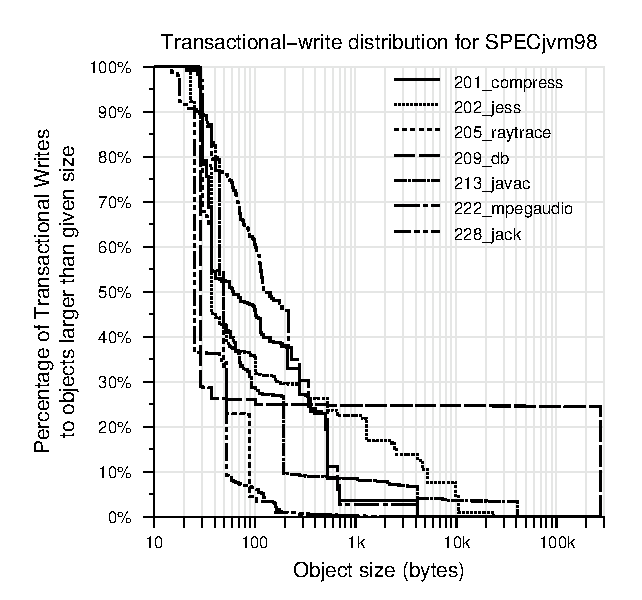
\includegraphics[width=2.25in,clip=true]{Figures/tr-w-all}%
\end{center}%
\caption{Proportion of transactional writes to objects equal to or
  smaller than a given size.}
\label{fig:tr-w}%
\end{figure}%
My software transactions implementation clones objects on
transactional writes, so that the previous state of the object can be
restored if the transaction aborts.  \figref{tr-w} shows the object
size distribution of transactional writes for SPECjvm98, and
indicates that over 10\% of writes may be to large objects.
Obviously the copying cost would be prohibitive.

My solution is to represent large objects as \defn{functional
  arrays}.  O'Neill and Burton \cite{ONeillBu97} give a fairly
inclusive overview of such algorithms; I've chosen Tyng-Ruey Chuang's
version \cite{Chuang94} of \emph{shallow binding}, which uses
randomized cuts to the version tree to limit the cost of a read to
$O(n)$ in the worst case.  Single-threaded accesses to the array are
$O(1)$.  Our use of functional arrays is single-threaded in the common
case, when transactions do not abort.  Chuang's scheme is attractive
because it limits the worst-case cost of an abort, with very little
added complexity.

Of course, Chuang's algorithm is not lock free.
The crucial operation is a rotation of a \emph{difference node} with the
main body of the array.  I will present a lock-free version of
Chaung's algorithm later.  I will begin by
reformulating transactions on objects in terms of concurrent
operations on functional arrays.

\section{Basic operations on functional arrays}
My large object support will use \emph{functional arrays} as
a building block.  Functional arrays are \emph{persistent}; that is,
after an element is updated both the new and the old contents of the
array are available for use.  Since arrays are simply maps from
integers (indexes) to values; any functional map datatype (for
example, a functional balanced tree) can be used to implement
functional arrays.

However, the distinguishing characteristic of an imperative array is its
theoretical complexity: $O(1)$ access or update of any element.
Implementing functional arrays with a functional balanced tree yields
$O(\lg n)$ worst-case access or update.\footnote{I will return to
consider operation complexity in \charef{large-obj}.}

For concreteness, functional arrays have the following three
operations defined:
\begin{itemize}
\item $\funcname{FA-Create}(n)$: Return an array $A$ of size $n$.  The
  contents of the array are initialized to zero.
\item $\funcname{FA-Update}(A, i, v)$: Return an array $A'$ which is
  functionally identical to array $A$ except that
  $\funcname{FA-Read}(A', i)=v$.
  Array $A$ is not destroyed and can be accessed further.
\item $\funcname{FA-Read}(A, i)$: Return $A(i)$ (that is, the
  value of the $i$th element of array $A$).
\end{itemize}
We allow any of these operations to \emph{fail}.  Failed operations
can be safely retried, as all operations are idempotent by definition.

For the moment, consider the following na{\"\i}ve implementation:
\begin{itemize}
\item $\funcname{FA-Create}(n)$: Return an ordinary imperative array of size
  $n$.
\item $\funcname{FA-Update}(A, i, v)$: Create a new imperative array
  $A'$ and copy the contents of $A$ to $A'$.  Set $A'[i]=v$. Return $A'$.
\item $\funcname{FA-Read}(A, i)$: Return $A[i]$.
\end{itemize}
This implementation has $O(1)$ read and $O(n)$ update, so it matches
the performance of imperative arrays only when $n=O(1)$.  I will
therefore call these \emph{small object functional arrays}.  Operations
in this implementation never fail.  Every operation is non-blocking
and no synchronization is necessary, since the imperative arrays are
never mutated after they are created.

\section{A single-object protocol}
\begin{figure}\centering
\includegraphics[width=3.25in,clip=true]{Figures/nb-single-obj}
\caption{Implementing non-blocking single-object concurrent operations
  with functional arrays.}
\label{fig:single-o}
\end{figure}
Given a non-blocking implementation of functional arrays, we can
construct a transaction implementation for single objects.  In
this implementation, fields of at most one object may be referenced
during the execution of the transaction.

I will consider the following two operations on objects:
\begin{itemize}
\item $\funcname{Read}(o, f)$: Read field $f$ of $o$.  We will assume that
  there is a constant mapping function which given a field name
  returns an integer index.  We will write the result of mapping $f$
  as \fref{f}{index}.  For simplicity, and without loss of generality,
  we will assume all fields are of equal size.
\item $\funcname{Write}(o, f, v)$: Write value $v$ to field $f$ of $o$.
\end{itemize}
All other operations on Java objects, such as method dispatch and type
interrogation, can be performed using the immutable {\tt type}
field in the object.  Because the {\tt type} field is never changed
after object creation, non-blocking implementations of operations on
the {\tt type} field are trivial.

As Figure~\ref{fig:single-o} shows, our single-object transaction
implementation represents objects as a pair, combining {\tt type} and a
reference to a functional array.  When not inside a transaction,
object reads and writes are implemented using the
corresponding functional array operation, with the array reference in
the object being updated appropriately:
\begin{itemize}
\item $\funcname{Read}(o, f)$:
  Return $\funcname{FA-Read}(\fref{o}{fields}, \fref{f}{index})$.
\item $\funcname{Write}(o, f, v)$: Replace \fref{o}{fields} with the
  result of \linebreak
  $\funcname{FA-Update}(\fref{o}{fields}, \fref{f}{index}, v)$.
\end{itemize}

The interesting cases are reads and writes inside a transaction.
At entry to our transaction which will access (only) object $o$, we
store \fref{o}{fields} in a local variable $u$.  We create another
local variable $u'$ which we initialize to $u$.  Then our read and
write operations are implemented as:
\begin{itemize}
\item $\funcname{ReadT}(o, f)$:
  Return $\funcname{FA-Read}(u', \fref{f}{index})$.
\item $\funcname{WriteT}(o, f, v)$:
  Update variable $u'$ to the result of \linebreak
  $\funcname{FA-Update}(u', \fref{f}{index}, v)$.
\end{itemize}

At the end of the transaction, we use Compare-And-Swap to atomically
set \fref{o}{fields} to $u'$ iff it contained $u$.  If the CAS fails,
we the transaction is aborted (we simply discard $u'$) and we retry.

With our na{\"\i}ve ``small object'' functional arrays, this implementation is
exactly the ``small object protocol'' of Herlihy \cite{Herlihy93}.
Herlihy's protocol is rightly criticized for an excessive amount of
copying.  I will address this with a better implementation of
functional arrays in Section~\ref{sec:large-obj}.
However, the restriction that only one object
may be referenced within a transaction is overly limiting.  I will
first fix this problem.

\section{Extension to multiple objects}
\begin{figure}[t]\centering
\includegraphics[width=3.25in,clip=true]{Figures/nb-multi-obj}
\caption[Data structures to support non-blocking multi-object
  concurrent operations.]{Data structures to support non-blocking multi-object
  concurrent operations.  Objects point to a linked list of versions,
  which reference transaction identifiers.  Versions created within the
  same execution of a transaction share the same transaction
  identifier.  Version structure also contain pointers to functional
  arrays, which record the values for the fields of the object.
  If no modifications have been made to the object, multiple versions
  in the list may share the same functional array.}
\label{fig:multi-o}
\end{figure}
\begin{figure}[p]
\sis%
\renewcommand{\>}{~~}%
\newcommand{\com}[1]{\hfill [{\sl #1}]}%
\begin{tabular}{l}%
$\funcname{Read}(o, f)$:\\
begin\\
retry:\\
\>$u \gets \fref{o}{versions}$ \\
\>$u' \gets \fref{u}{next}$ \\
\>$s  \gets \fref{\fref{u}{owner}}{status}$ \\
\>if ($s=\text{\sl DISCARDED}$) \com{Delete DISCARDED?}\\
\>\>CAS$(u, u', \addr{\fref{o}{versions}})$\\
\>\>goto retry \\
\>else if ($s=\text{\sl COMPLETE}$)\\
\>\>$a \gets \fref{u}{fields}$ \com{$u$ is COMPLETE}\\
\>\>$\fref{u}{next} \gets \text{\bf null}$ \com{Trim version list}\\
\>else\\
\>\>$a \gets \fref{u'}{fields}$ \com{$u'$ is COMPLETE}\\
\>return $\funcname{FA-Read}(a, \fref{f}{index})$ \com{Do the read}\\
end\\
\\
$\funcname{ReadT}(o, f)$:\\
begin\\
\>$u \gets \fref{o}{versions}$\\
\>if ($\var{oid} = \fref{u}{owner}$) \com{My OID should be first}\\
\>\>return $\funcname{FA-Read}(\fref{u}{fields}, \fref{f}{index})$
\com{Do the read}\\
\>else \com{Make me first!}\\
\>\>$u' \gets \fref{u}{next}$\\
\>\>$s  \gets \fref{\fref{u}{owner}}{status}$\\
\>\>if ($s=\text{\sl DISCARDED}$) \com{Delete DISCARDED?}\\
\>\>\>CAS$(u, u', \addr{\fref{o}{versions}})$\\
\>\>else if ($\fref{\var{oid}}{status}=\text{\sl DISCARDED}$)
\com{Am I alive?}\\
\>\>\>fail\\
\>\>else if ($s=\text{\sl IN-PROGRESS}$) \com{Abort IN-PROGRESS?}\\
\>\>\>CAS$(s, \text{\sl DISCARDED}, \addr{\fref{\fref{u}{owner}}{status}})$\\
\>\>else \com{Link new version in:} \\
\>\>\>$\fref{u}{next} \gets \text{\bf null}$ \com{Trim version list}\\
\>\>\>$u' \gets \text{new \tt Version}(\var{oid}, u, \text{\bf null})$
\com{Create new version}\\
\>\>\>if (CAS$(u, u', \addr{\fref{o}{versions}}) \neq \text{\sl FAIL}$)\\
\>\>\>\>$\fref{u'}{fields} \gets \fref{u}{fields}$ \com{Copy old fields}\\
\>\>goto retry\\
end\\
\end{tabular}
\caption{\funcname{Read} and \funcname{ReadT} implementations for the
  multi-object protocol.}\label{fig:reads}
\end{figure}

\begin{figure}[p]
\sis%
\renewcommand{\>}{~~}%
\newcommand{\com}[1]{\hfill [{\sl #1}]}%
\begin{tabular}{l}%
$\funcname{Write}(o, f, v)$:\\
begin\\
retry:\\
\>$u  \gets \fref{o}{versions}$\\
\>$u' \gets \fref{u}{next}$\\
\>$s  \gets \fref{\fref{u}{owner}}{status}$\\
\>if ($s=\text{\sl DISCARDED}$) \com{Delete DISCARDED?}\\
\>\>CAS$(u, u', \addr{\fref{o}{versions}})$\\
\>else if ($s=\text{\sl IN-PROGRESS}$) \com{Abort IN-PROGRESS?}\\
\>\>CAS$(s, \text{\sl DISCARDED}, \addr{\fref{\fref{u}{owner}}{status}})$\\
\>else \com{$u$ is COMPLETE}\\
\>\>$\fref{u}{next} \gets \text{\bf null}$ \com{Trim version list}\\
\>\>$a \gets \fref{u}{fields}$\\
\>\>$a' \gets \funcname{FA-Update}(a, \fref{f}{index}, v)$\\
\>\>if (CAS$(a, a', \addr{\fref{u}{fields}}) \neq \text{\sl FAIL}$)
\com{Do the write}\\
\>\>\>return \com{Success!}\\
\>goto retry\\
end\\
\\
$\funcname{WriteT}(o, f, v)$:\\
begin\\
\>$u  \gets \fref{o}{versions}$\\
\>if ($oid = \fref{u}{owner}$) \com{My OID should be first}\\
\>\>$\fref{u}{fields} \gets \funcname{FA-Update}(\fref{u}{fields}, \fref{f}{index}, v)$\com{Do write}\\
\>else \com{Make me first!}\\
\>\>$u' \gets \fref{u}{next}$\\
\>\>$s  \gets \fref{\fref{u}{owner}}{status}$\\
\>\>if ($s=\text{\sl DISCARDED}$) \com{Delete DISCARDED?}\\
\>\>\>CAS$(u, u', \addr{\fref{o}{versions}})$\\
\>\>else if ($\fref{\var{oid}}{status}=\text{\sl DISCARDED}$)
\com{Am I alive?}\\
\>\>\>{\it fail}\\
\>\>else if ($s=\text{\sl IN-PROGRESS}$) \com{Abort IN-PROGRESS?}\\
\>\>\>CAS$(s, \text{\sl DISCARDED}, \addr{\fref{\fref{u}{owner}}{status}})$\\
\>\>else \com{Link new version in:} \\
\>\>\>$\fref{u}{next} \gets \text{\bf null}$ \com{Trim version list}\\
\>\>\>$u' \gets \text{new \tt Version}(\var{oid}, u, \text{\bf null})$
\com{Create new version}\\
\>\>\>if (CAS$(u, u', \addr{\fref{o}{versions}}) \neq \text{\sl FAIL}$)\\
\>\>\>\>$\fref{u'}{fields} \gets \fref{u}{fields}$ \com{Copy old fields}\\
\>\>goto retry\\
end\\
\end{tabular}
\caption{\funcname{Write} and \funcname{WriteT} implementations for the
  multi-object protocol.}\label{fig:writes}
\end{figure}

I extend the implementation to allow the fields of any number of
objects to be accessed during the transaction.
Figure~\ref{fig:multi-o} shows our new object representation.
Objects consist of two slots, and the first represents the immutable
{\tt type}, as before.  The second field, {\tt versions}, points to a
linked list of {\tt Version} structures.  The {\tt Version} structures
contain a pointer {\tt fields} to a functional array, and a pointer
{\tt owner} to an \emph{transaction identifier}.  The transaction
identifier contains a single field, {\tt status}, which can be set to
one of three values: \textsl{COMMITTED}, \textsl{IN-PROGRESS}, or
\textsl{ABORTED}.  When the transaction identifier is created, the
status field is initialized to \textsl{IN-PROGRESS}, and it will be
updated exactly once thereafter, to either \textsl{COMMITTED} or
\textsl{ABORTED}.  A \textsl{COMMITTED} transaction identifier never
later becomes \textsl{IN-PROGRESS} or \textsl{ABORTED}, and
a \textsl{ABORTED} transaction identifier never becomes
\textsl{COMMITTED} or \textsl{IN-PROGRESS}.

We create an transaction identifier when we begin or restart a transaction
and place it in a local variable \emph{tid}.  At the end of the
transaction, we use CAS to set \fref{\var{tid}}{status} to
{\sl COMMITTED} iff it was {\sl IN-PROGRESS}.  If the CAS is successful,
the transaction has also executed successfully; otherwise
$\fref{\var{tid}}{status}=\text{\sl ABORTED}$ (which indicates that
our transaction has been aborted) and we must back off and retry.
All {\tt Version} structures
created while in the transaction will reference \emph{tid} in
in their {\tt owner} field.

Semantically, the current field values for the object will be given by
the first version in 
the versions list whose transaction identifier is {\sl COMMITTED}.
This allows us to link {\sl IN-PROGRESS} versions in at the head of
multiple objects' versions lists and atomically change the values of
all these objects by setting the one common transaction identifier to
{\sl COMMITTED}.  We only allow one {\sl IN-PROGRESS} version on the
versions list, and it must be at the head, so
before we can link a new version at the head we
must ensure that every other version on the list is {\sl ABORTED} or
{\sl COMMITTED}.

Since we will never look past the first {\sl COMMITTED} version in the
versions list, we can free all versions past that point.  In our
presentation of the algorithm, we do this by explicitly setting the
{\tt next} field of every {\sl COMMITTED} version we see to {\bf null};
this allows the versions past that point to be garbage collected.
An optimization would be to have the garbage collector do the list
trimming for us when it does a collection.
% always must read u.next before u.owner.status to ensure we don't
% get caught with a null pointer from a version that just committed.

We don't want to inadvertently chase the null {\tt next} pointer
of a {\sl COMMITTED} version, so we always load the {\tt next}
field of a version \emph{before} we load {\tt owner.status}.  Since
the writes occur in the reverse order ({\sl COMMITTED} to
{\tt owner.status}, then {\bf null} to {\tt next}) we have ensured that
our {\tt next} pointer is valid whenever the status is not {\sl COMMITTED}.

We begin an atomic method with \funcname{TransStart} and attempt to
complete an atomic method with \funcname{TransEnd}.  They are defined as
follows:
\begin{itemize}
\item $\funcname{TransStart}$: create a new transaction identifier, with
  its status initialized to {\sl IN-PROGRESS}.  Assign it to the
  thread-local variable \var{tid}.
\item $\funcname{TransEnd}$:
  If
 $$\text{CAS}(\text{\sl IN-PROGRESS}, \text{\sl COMMITTED},
             \addr{\fref{\var{tid}}{status}})$$
  is successful, the transaction as a whole has completed successfully,
  and can be linearized at the location of the CAS.
  Otherwise, the transaction has been aborted.  Back off and retry from
  \funcname{TransStart}.
\end{itemize}
Pseudo-code describing \funcname{Read}, \funcname{Write}, \funcname{ReadT},
and \funcname{WriteT} is presented in Figures~\ref{fig:reads} and
\ref{fig:writes}.  In the absence of contention, all operations take
constant time plus an invocation of \funcname{FA-Read} or
\funcname{FA-Update}.

\section{Lock-free functional arrays}\label{sec:large-obj}
\begin{figure}\centering
\includegraphics[width=6in,clip=true]{Figures/chuang}
\caption{Shallow binding scheme for functional arrays, from
  \cite[Figure~1]{Chuang94}.}
\label{fig:chuang}
\end{figure}
In this section I will present a lock-free implementation of functional
arrays with $O(1)$ performance in the absence of contention.  This
will complete our implementation of non-blocking transactions for Java.

There have been a number of proposed implementations of functional
arrays, starting from the ``classical'' functional binary tree
implementation.  O'Neill and Burton \cite{ONeillBu97} give a fairly
inclusive overview.  Functional array implementations fall generally
into one of three categories: \emph{tree-based}, \emph{fat-elements},
or \emph{shallow-binding}.

Tree-based implementations typically have a logarithmic term in their
complexity.  The simplest is the persistent binary tree with $O(\ln
n)$ look-up time; Chris Okasaki 
\cite{Okasaki95} has implemented a purely-functional random-access list
with $O(\ln i)$ expected lookup time, where $i$ is the index of the
desired element.

Fat-elements implementations have per-element data structures indexed
by a master array. Cohen \cite{Cohen84} hangs a list of
versions from each element in the master array.
O'Neill and Burton \cite{ONeillBu97}, in a more sophisticated
technique, hang a splay tree off each element and achieve $O(1)$
operations for single-threaded use, $O(1)$ amortized cost when
accesses to the array are ``uniform'', and $O(\ln n)$ amortized worst
case time. 

Shallow binding was introduced by Baker \cite{Baker78} as a method to
achieve fast variable lookup in Lisp environments.  Baker clarified
the relationship to functional arrays in \cite{Baker91}.  Shallow
binding is also called \emph{version tree arrays}, \emph{trailer
  arrays}, or \emph{reversible differential lists}.  A typical
drawback of shallow binding is that reads may take $O(u)$ worst-case
time, where $u$ is the number of updates made to the array.  Tyng-Ruey
Chuang \cite{Chuang94} uses randomized cuts to the version tree to limit
the cost of a read to $O(n)$ in the worst case.  Single-threaded
accesses are $O(1)$.

Our use of functional arrays is single-threaded in the common case,
when transactions do not abort.  Chuang's scheme is attractive because
it limits the worst-case cost of an abort, with very little added
complexity.   In this section I will present a lock-free version of
Chuang's randomized algorithm.

In shallow binding, only one version of the functional array (the
\emph{root}) keeps its contents in an imperative array (the
\emph{cache}).   Each of the other versions is represented as a path
of \emph{differential nodes}, where each node describes the
differences between the current array and the previous array.  The
difference is represented as a pair \tuple{\text{\it index},\text{\it value}},
representing the new value to be stored at the specified index.
All paths lead to the root.  An update to the functional array is
simply implemented by adding a differential node pointing to the array it is
updating.

The key to constant-time access for single-threaded use is provided by the read
operation.  A read to the root simply reads the appropriate value from
the cache.  However, a read to a differential node triggers a series
of rotations which swap the direction of differential nodes and result
in the current array acquiring the cache and becoming the new root.
This sequence of rotations is called \emph{re-rooting}, and is
illustrated in Figure~\ref{fig:chuang}.  Each rotation
exchanges the root nodes for a differential node pointing to it, after
which the differential node becomes the new root and the root becomes
a differential node pointing to the new root. The cost of a read is
proportional to its re-rooting length, but after the first read
accesses to the same version are $O(1)$ until the array is re-rooted again.

Shallow binding performs badly if read operations ping-pong between two
widely separated versions of the array, as we will continually
re-root the array from one version to the other.
Chuang's contribution is to provide for \emph{cuts} to the chain of
differential nodes: once in a while we clone the cache and create a
new root instead of performing a rotation.  This operation takes
$O(n)$ time, so we amortize it over $n$ operations by randomly
choosing to perform a cut with probability $1/n$.

\begin{figure}\centering%
\includegraphics[width=5.5in,clip=true]{Figures/funarr}
\caption[Atomic steps in $\funcname{FA-Rotate}(B)$.]%
 {Atomic steps in $\funcname{FA-Rotate}(B)$.  Time proceeds top-to-bottom
  on the left hand side, and then top-to-bottom on the right.
  Array $A$ is a root node, and $\funcname{FA-Read}(A, x)=z$.
  Array $B$ has the almost the same contents as $A$, but
  $\funcname{FA-Read}(B, x)=y$.}
\label{fig:funarr}
\end{figure}

\begin{figure}\centering%
\sis%
\renewcommand{\>}{~~}%
\newcommand{\com}[1]{\hfill [{\sl #1}]}%
\begin{tabular}{l}%
$\funcname{FA-Update}(A, i, v)$:\\
begin\\
\>$d \gets \text{new DiffNode}(i, v, A)$\\
\>$A'\gets \text{new Array}(\fref{A}{size}, d)$\\
\>return $A'$\\
end\\
\\
$\funcname{FA-Read}(A, i)$:\\
begin\\
retry:\\
\>$d_C \gets \fref{A}{node}$\\
\>if $d_C$ is a cache, then\\
\>\>$v \gets \fref{A}{node}[i]$\\
\>\>if $(\fref{A}{node} \neq d_C)$\com{consistency check}\\
\>\>\>goto retry\\
\>\>return $v$\\
\>else\\
\>\>\funcname{FA-Rotate}(A)\\
\>\>goto retry\\
end\\
\end{tabular}
\caption{Implementation of lock-free functional array using shallow
  binding and randomized cuts (part 1).}
\label{fig:fun-impl1}
\end{figure}
\begin{figure}\centering%
\sis%
\renewcommand{\>}{~~}%
\newcommand{\com}[1]{\hfill [{\sl #1}]}%
\begin{tabular}{l}%
$\funcname{FA-Rotate}(B)$:\\
begin\\
retry:\\
\>$d_B \gets \fref{B}{node}$\com{step (1): assign names as per Figure~\ref{fig:funarr}.}\\
\>$A \gets \fref{d_B}{array}$\\
\>$x \gets \fref{d_B}{index}$\\
\>$y \gets \fref{d_B}{value}$\\
\>$z \gets \funcname{FA-Read}(A, x)$\com{rotates A as side effect}\\
\\
\>$d_C \gets \fref{A}{node}$\\
\>if $d_C$ is not a cache, then \\
\>\>goto retry\\
\\
\>if $(0 = (\text{random} \bmod \fref{A}{size}))$\com{random cut}\\
\>\>$d_C' \gets \text{copy of }d_C$\\
\>\>$d_C'[x] \gets y$\\
\>\>$s\gets\text{DCAS}(d_C, d_C, \addr{\fref{A}{node}}, d_B, d_C', \addr{\fref{B}{node}})$\\
\>\>if $(s \neq \text{\sl SUCCESS})$ goto retry\\
\>\>else return\\
\\
\>$C \gets \text{new Array}(\fref{A}{size}, d_C)$\\
\>$d_A \gets \text{new DiffNode}(x, z, C)$\\
\\
\>$s \gets \text{CAS}(d_C, d_A, \addr{\fref{A}{node}})$\com{step (2)}\\
\>if $(s\neq \text{\sl SUCCESS})$ goto retry\\
\\
\>$s\gets\text{CAS}(A, C, \addr{\fref{d_B}{array}})$\com{step (3)}\\
\>if $(s\neq \text{\sl SUCCESS})$ goto retry\\
\\
\>$s \gets\text{CAS}(C, B, \addr{\fref{d_A}{array}})$\com{step (4)}\\
\>if $(s\neq \text{\sl SUCCESS})$ goto retry\\
\\
\>$s \gets \text{DCAS}(z, y, \addr{d_C[x]},  d_C, d_C, \addr{\fref{C}{node}})$\com{step (5)}\\
\>if $(s\neq \text{\sl SUCCESS})$ goto retry\\
\\
\>$s \gets \text{DCAS}(d_B, d_C, \addr{\fref{B}{node}}, d_C, {\bf nil}, \addr{\fref{C}{node}})$\com{step (6)}\\
\>if $(s\neq \text{\sl SUCCESS})$ goto retry\\
end\\
\end{tabular}
\caption{Implementation of lock-free functional array using shallow
  binding and randomized cuts (part 2).}
\label{fig:fun-impl2}
\end{figure}

Figure~\ref{fig:funarr} shows the data structures used for the
functional array implementation, and the series of atomic steps used
to implement a rotation.  The {\tt Array} class represents a
functional array; it consists of a {\tt size} for the array and a
pointer to a {\tt Node}.  There are two types of nodes: a {\tt
  CacheNode} stores a value for every index in the array, and a {\tt
  DiffNode} stores a single change to an array.  {\tt Array} objects
which point to {\tt CacheNode}s are roots.

In step 1 of the figure, we have a root array $A$ and an
array $B$ whose differential node $d_B$ points to $A$.  The functional
arrays $A$ and $B$ differ in one element: element $x$ of $A$ is $z$,
while element $x$ of $B$ is $y$.  We are about to rotate $B$ to give
it the cache, while linking a differential node to $A$.

Step 2 shows our first atomic action.  We have created a new {\tt
  DiffNode} $d_A$ and a new {\tt Array} $C$ and linked them between
$A$ and its cache.  The {\tt DiffNode} $d_A$ contains the value for
element $x$ contained in the cache, $z$, so there is no change in
the value of $A$.

We continue swinging pointers until step 5, when can finally set
the element $x$ in the cache to $y$.  We perform this operation with a
DCAS operation which checks that $\fref{C}{node}$ is still pointing to
the cache as we expect.  Note that a concurrent rotation would swing
$\fref{C}{node}$ in its step 1.  In general, therefore, the location
pointing to the cache serves as a reservation on the cache.

Thus in step 6 we need to again use DCAS to simultaneously swing
$\fref{C}{node}$ away 
from the cache as we swing $\fref{B}{node}$ to point to the cache.

Figures~\ref{fig:fun-impl1} and \ref{fig:fun-impl2} present pseudocode
for \funcname{FA-Rotate}, \funcname{FA-Read}, and
\funcname{FA-Update}.  Note that \funcname{FA-Read} also uses the
cache pointer as a reservation, double-checking the cache pointer
after it finishes its read to ensure that the cache hasn't been stolen
from it.

Let us now consider cuts, where \funcname{FA-Read} clones the cache
instead of performing a rotation.   Cuts also check the cache pointer
to protect against concurrent rotations.  But what if the cut occurs
while a rotation is mutating the cache in step 5?  In this case the
only array adjacent to the root is $B$, so the cut must be occurring
during an invocation of $\funcname{FA-Rotate}(B)$.  But then the
differential node $d_B$ will be applied after the cache is copied,
which will safely overwrite the mutation we were concerned about.

Note that with hardware support for small transactions \cite{HerlihyMo93}
we could cheaply perform the entire rotation atomically, instead of
using this six-step approach.


%% \section{Optimizations}
%% Re-rooting is the most complicated part of the functional array
%% algorithm.  It can be optimized in a number of ways.  For example,

%% %unsync rotate for transaction-local data.
%% The first is to recognize that some array versions can only be seen by
%% a single thread.  In particular, when we are working on an {\sl
%%   IN-PROGRESS} operation, all array versions which it creates are
%% unreachable from other threads until the operation is committed.
%% We can add a field {\tt creator} to the {\tt Array} object which records what
%% operation created that version.  If the {\tt creator} field of both
%% $A$ and $B$ contains our own \var{tid} when we begin a rotate, we know
%% that these versions are both thread local

%% .. uh, no.  This doesn't work.

%% % scales method of tagging fields.

\section{Performance of functional array implementation}

XXX: continue previous microbenchmarks, as function of object size.

%%%%%%%%%%%%%%%%%%%%%


% LocalWords:  Promela microbenchmark Hennessy PowerPC setjmp longjmp runtime
% LocalWords:  subsumption
